% This file should be replaced with your file with thesis content.
%=========================================================================
% Authors: Michal Bidlo, Bohuslav Křena, Jaroslav Dytrych, Petr Veigend and Adam Herout 2019, Ondřej Zobal 2024

% For compilation piecewise (see projekt.tex), it is necessary to uncomment it and change
% \documentclass[../projekt.tex]{subfiles}
% \begin{document}

%% ###                            
%%  #  #    # ##### #####   ####  
%%  #  ##   #   #   #    # #    # 
%%  #  # #  #   #   #    # #    # 
%%  #  #  # #   #   #####  #    # 
%%  #  #   ##   #   #   #  #    # 
%% ### #    #   #   #    #  ####  

\chapter{Introduction}

%% Context and Rationale
In the fast-paced field of software development, maintaining code quality and readability is crucial. This thesis introduces a tool for automatic code refactoring aid using Large Language Models (LLM), which aims to enhance code readability, quality, as well as the overall developer experience.  

Most contemporary tools lean heavily on chatting with generative AI assistants\footnote{Among those most popular by developers are copilot and chatGPT. Copilot offers next token prediction and chatting and is powered by GPT-3.5, chatGPT can only do chatting and is powered by GPT-3.5 and GPT-4}; these are usually very flexible, often able to perform operations they never directly saw in their training data; however, due to their broad focus, they often lack mastery.  Additionally, chatting doesn't make for the best workflow, especially when dealing with simple tasks that need to be performed often. Despite the recent language modeling boom, IDEs still lack more integrated AI tools for performing simple chores.

%% Specific Challenges Addressed
The aim of this thesis is to design, implement, and evaluate a \emph{VS Code/Code-OSS}\footnote{Code-OSS is a Free project developed by Microsoft, and Microsoft Visual Studio Code (VS Code for short) is its most popular distribution.} extension called \emph{CodeImprove} that uses AI to assist Python developers by enhancing code quality. Specifically, the extension will attempt to automate the generation of docstrings and comments, suggest more fitting variable names, and identify as well as fix common coding errors. 

%% Innovative Approach
To address these challenges while retraining reasonable hardware requirements, this thesis uses the Longformer. This sparse attention transformer model saves memory by focusing on a smaller window of code at a time. This paper also experiments with quantized low-rank adaptation, a different approach for reducing the memory use of large language models.

%% Structure of the Thesis
The thesis is organized as follows: An exploration of the theory behind contemporary state-of-the-art natural language processors is conducted over the next three chapters, ranging from neurons to the transformer model. The technologies employed in this project will be presented, along with the training data utilized for model creation, and are explained. Subsequently, the manner in which the models were trained is showcased, followed by details of the implementation of the extensions. Lastly, the evaluation of performance is examined, and the results are summarized.

%% ===================================================
%%  _   _                      _   _   _      _
%% | \ | | ___ _   _ _ __ __ _| | | \ | | ___| |_ ___
%% |  \I |/ _ \ | | | '__/ _` | | |  \I |/ _ \ __/ __|
%% | |\  |  __/ |_| | | | (_| | | | |\  |  __/ |_\__ \
%% |_| \_|\___|\__,_|_|  \__,_|_| |_| \_|\___|\__|___/
%% ===================================================

%%% LARGE LANGUAGE MODELS

\chapter{Neural networks}
\label{sec:neural_networks}

This chapter will go over the theory behind \emph{neural networks (NN)}, also sometimes called \emph{Artificial Neural Networks} (ANN), which are a cornerstone in machine learning. Neural networks enable computers to gain intuition in complex tasks by learning from vast amounts of data, relying solely on matrix multiplication and a handful of other simple mathematical functions for generating their predictions.

Neural networks are a branch of artificial intelligence. They are computational models designed to recognize patterns and solve complex problems. Neural networks can learn from datasets featuring examples of problems with solutions. Later chapters will explain how neural networks can be used to intelligently transform and generate textual content \ref{sec:llm}. Information in this chapter is based on\,\cite{DeepLearning2016}.

\medskip

Neural networks are a model that \emph{approximates} a given function $y = f^{*}(x)$ by defining a function $y = f(x,\theta)$ and learning the value $\theta$ so that the outputs of $f$ are as close as possible to the outputs of~$f^{*}$.

Neural networks can be represented as a composition of various functions within a directed graph. This chapter will focus on \emph{feedforward networks} that are an \emph{acyclic} variant of neural networks, meaning they do not contain feedback connections to previous layers. Some feedforward network $f(x)$ can be characterized as $f(x) = f_{n}(f_{2}(f_{1}(x)))$ as shown in \ref{fig:nn-functional}.

\begin{figure}[ht]
  \centering
  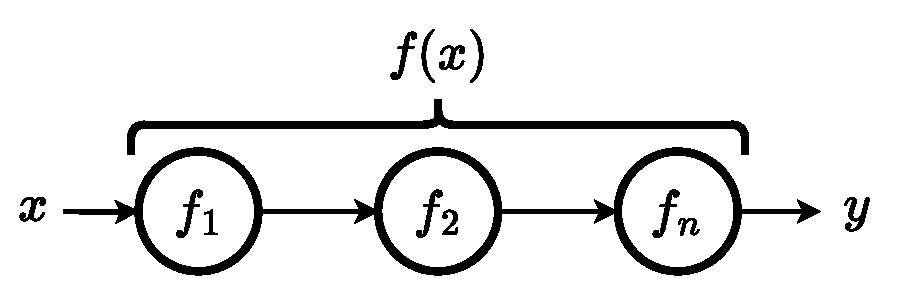
\includegraphics[width=0.55\textwidth]{neural-net-functional.pdf}
  \caption{$x$ is an input passed to the first layer $f_{1}$. Its output is passed to the second layer $f_{2}$ and so on until it arrives at $f_{n}$, which is the last layer, and its output is the output of the model.}
  \label{fig:nn-functional}
\end{figure}

Dataset defines \emph{inputs} and \emph{labels} representing $x$ and $f(x)$, respectively. In a neural network, inputs correspond to the value of the \emph{input layer} and labels to the desired value of the \emph{output layer}. Any other layers between them do not have their values bound by the dataset; because of this, they are called \emph{hidden layers}.

Inputs, labels, and outputs of individual layer functions are usually \emph{vector-valued}. The dimensionality of a layer is called \emph{width}. Each unit in these vectors can be visualized as a node that operates in parallel to other nodes within the same layer. These nodes are called \emph{neurons} for their functional similarity to their biological counterparts.

\medskip
The goal of using hidden layers is for the network to be able to split a potentially complex task into more manageable sub-tasks that can then be divided between the layers. However, by only using linear operations, the network's learning potential is limited to only observing linear relationships in the data. This can be solved by employing a \emph{non-linear function} to transform the output of our linear layer. This function is called an \emph{activation function}.

The activation function does not require its own trainable parameters, and the function itself does not need to be very complex. The most popular non-linear function is \emph{ReLU}, which consists of a constant function that changes into a linear function for $x > 0$ as pictured in figure \ref{fig:relu}.

The final output value of a neuron is called an \emph{activation}.

\begin{figure}[ht]
  \centering
  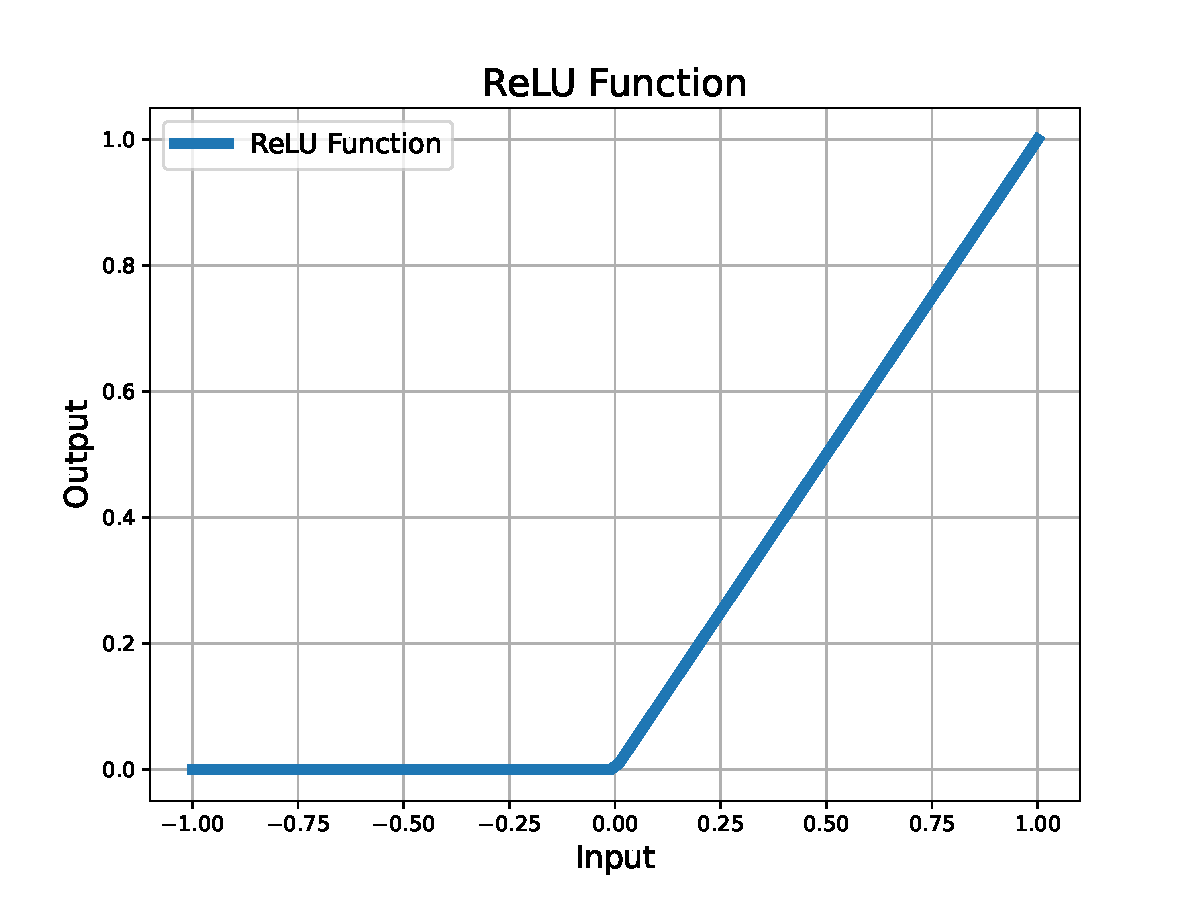
\includegraphics[width=0.7\textwidth]{relu.pdf}
  \caption{ReLU function graph. It is a primitive yet powerful activation function with great results with models that use a large number of layers.}
  \label{fig:relu}
\end{figure}

\begin{figure}[ht]
  \centering
  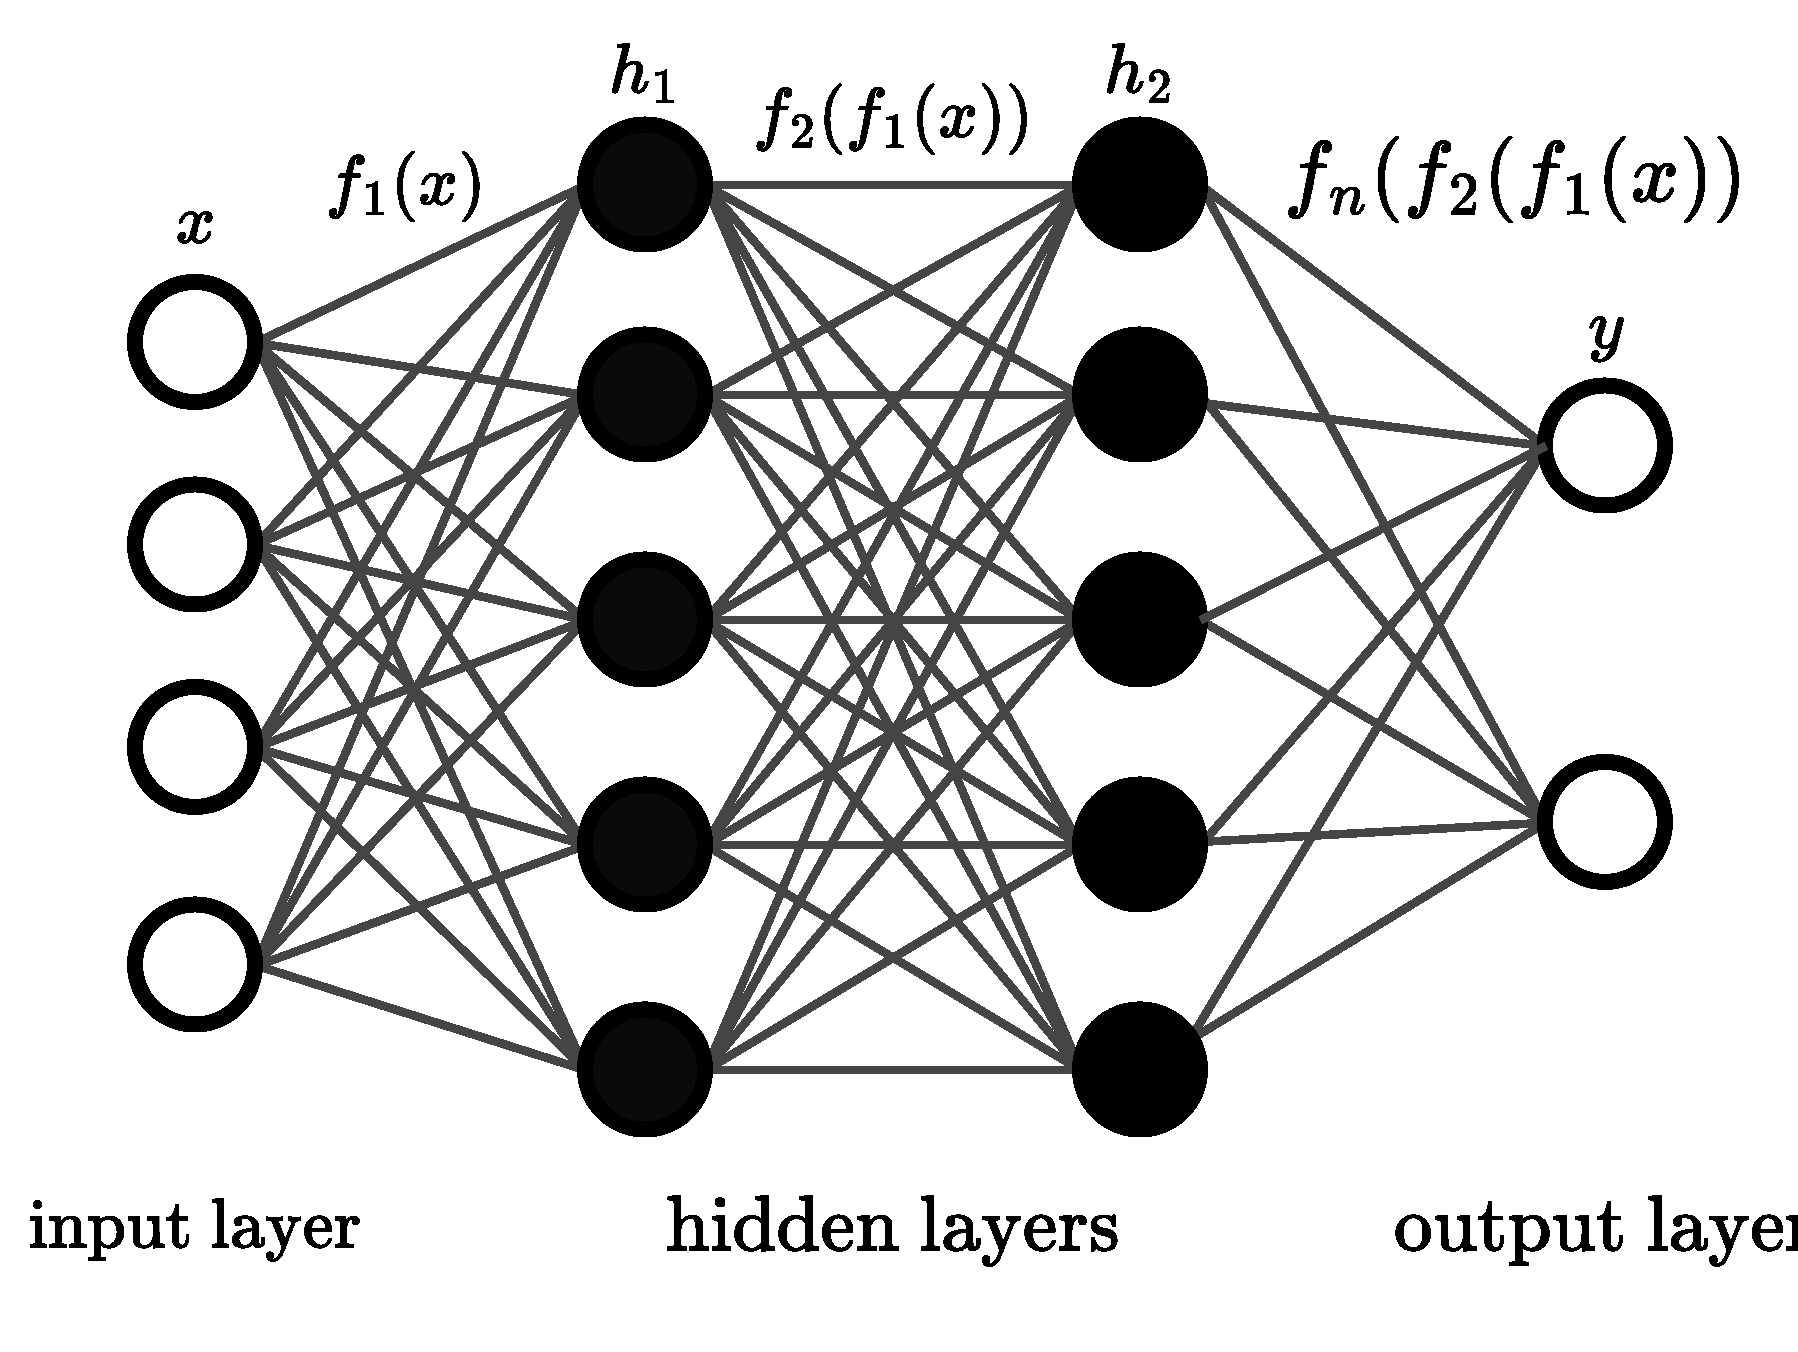
\includegraphics[width=0.65\textwidth]{neural-net.pdf}
  \caption{A 4 layer feedforward network modeling $y = f_{n}(f_{2}(f_{1}(x)))$. The activations of the input layer are set to the value $x$. The values pass from left to right through hidden layers $h_{1}$, $h_{2}$, and finally, the output layer $y$ whose activations represent the model's prediction.}
  \label{fig:ff}
\end{figure}

\medskip
The linear layer is a cornerstone of neural networks. It computes a linear transformation like this:

\begin{equation}
  y = x^{T} \cdot w + b
\end{equation}

where $w$ and $b$ together represent $\theta$. $w$ is commonly referred to as a \emph{weight} and serves to dim or amplify the activation coming from a particular connection, and $b$ \emph{bias} gives the neuron a tendency towards being more or less activated. $x^{T}$ is a transposed vector of activations from neurons of the previous layer, and finally $y$ it the output vector of activations.

Another important layer is the non-linear layer. Which is essentially the same as the linear transformation, except a non-linear function processes its output. Activation of a non-linear neuron can be computed like this:
\begin{equation}
\text{Activation} = \phi\left(\sum_{i=1}^{n} W_{i}x_{i} + b\right)
\label{eq:non-linear}
\end{equation}

$\phi$ is an activation function (such as ReLU), $n$ is the total number of connections from the previous layer to this neuron, $W_{i}$ is the weight of a connection, $x_{i}$ the activation of the connected neuron, and $b$ is the bias value of this neuron. Also see equivalent block diagram \ref{fig:neuron}.

\begin{figure}[ht]
  \centering
  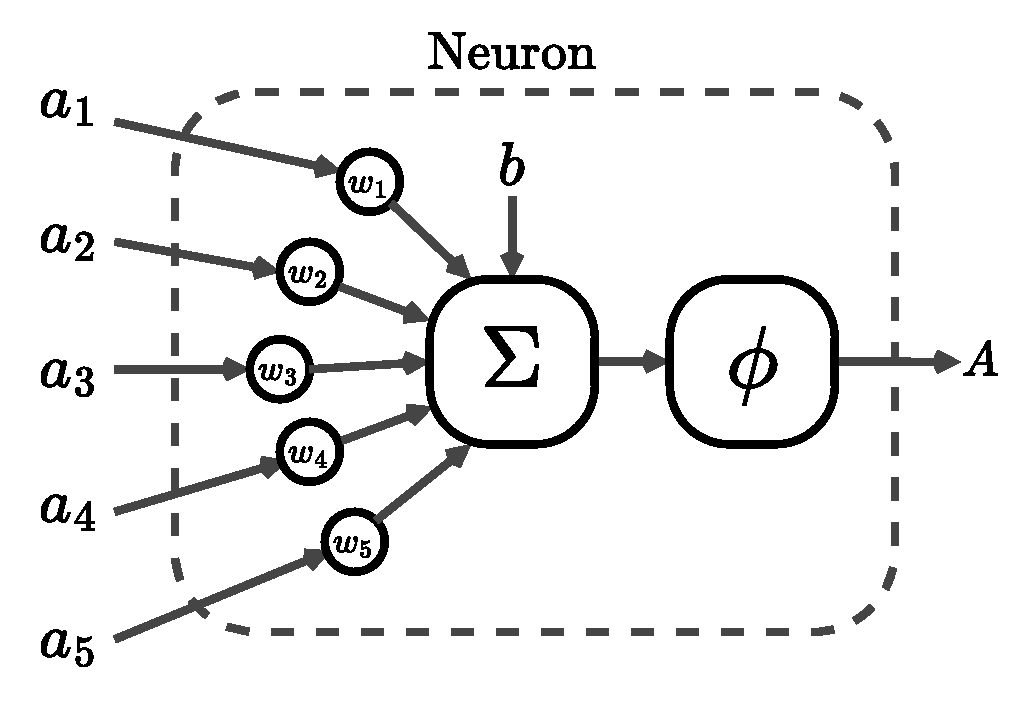
\includegraphics[width=0.6\textwidth]{neuron-connections.pdf}
  \caption{Block diagram of neuron activation calculation, equivalent to equation \ref{eq:non-linear}. $a_{1-5}$ are activations from all neurons in the previous layer. $a_{1-5}$ each get multiplied by their respective weights $w_{1-5}$ and the results are summed together with a bias parameter $b$. This sum is then processed by an activation function $\phi$, whose output is the neuron's activation. }
  \label{fig:neuron}
\end{figure}

\subsection{Training Neural Networks}

An obvious challenge when working with a neural network is obtaining suitable values for $\theta$. One approach used historically is manual tuning with the help of field experts. This approach is problematic as it requires extensive amounts of time and effort. And once training is done, very little progress can be shared with projects from different domains.

The model is trained by first running an inference. This is called the \emph{forward pass}. During the forward pass, the state of every layer is saved in a \emph{computational graph}. A \emph{cost function} is then used to calculate an error score between the model's output and the labels. This value is called a \emph{loss}. An \emph{optimization algorithm} such as \emph{back-propagation}\,\cite{BackProp1986} takes the computational graph obtained during the forward pass and, with the help of the \emph{chain rule}, computes gradients for each function, starting from the loss calculation, and going all the way to the input layer as shown in \ref{fig:back-prop}; this is called a \emph{backward pass}.

Naturally, the gradient represents the direction in which the parameter $\theta$ needs to be adjusted to increase the loss value, so by subtracting a fraction of the gradient from parameters $\theta$, the model's performance on the current sample improves. This is called \emph{gradient descend}. This process repeats until the model stops improving. Before the training starts, the parameters $\theta$ are typically initialized with random noise of low yet non-zero values.

\begin{figure}[H]
  \centering
  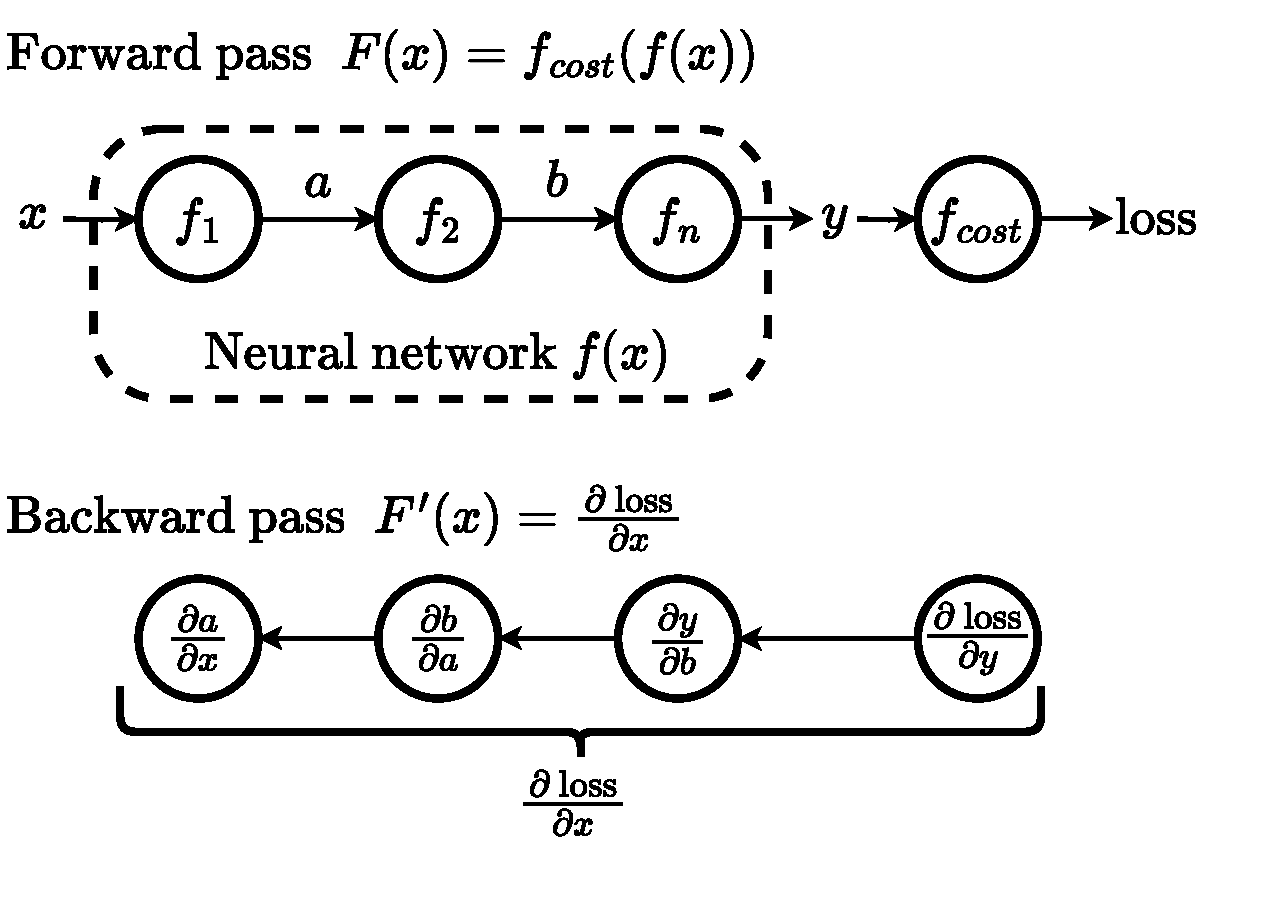
\includegraphics[width=0.75\textwidth]{neural-net-backprop.pdf}
  \caption{Forward pass and backward pass are shown side by side. During the forward pass $F(x)$, the function of the neural network $f(x)$ is computed along with its loss using $f_{cost}(f(x))$. Gradients can be obtained by deriving the forward pass $F'(x)$. By repeatedly applying the chain rule, the gradient for each function is calculated from the last to the first layer.}
  \label{fig:back-prop}
\end{figure}

The most popular cost function is cross-entropy between the model's outputs and labels. A form of cross-entropy that is widely used in multi-class classification tasks is the \emph{negative log likelihood} of an output layer with softmax\footnote{Softmax normalizes neuron activation in a layer so that their sum is $1$.} applied against the labels.

The negative log-likelihood is calculated as follows:

\begin{equation}
  \text{loss} = -\sum_{i=1}^{N} \log(p(y_i))
\end{equation}

$N$ is the number of processed samples, $y_{i}$ is the label value for $i^{th}$ sample, $p(y_i)$ is the predicted value for $i^{th}$ sample.

The network's architecture is integral to its performance. The ideal configuration will differ between applications. Configuration options include the number and types of layers, as well as the number of neurons inside them, the learning rate (gradient multiplier), and various regularization techniques.

\medskip
To make the neural network useful outside of the training examples, it is necessary to ensure that the model is only learning general patterns in the data and not memorizing the individual samples. Performance on unseen data can be tracked with an \emph{evaluation dataset} that contains unique samples and periodically runs inference on it without optimizing. A situation where the performance on the training dataset continues to improve, but the performance on the evaluation dataset remains stagnant or worsens is called \emph{overfitting}.

The opposite would be \emph{underfitting}, where the model stops improving before outputting satisfactory results.

%% ===========================
%%  ____        _
%% |  _ \  __ _| |_ __ _
%% | | | |/ _` | __/ _` |
%% | |_| | (_| | || (_| |
%% |____/ \__,_|\__\__,_|
%%  ____                                     _        _   _
%% |  _ \ ___ _ __  _ __ ___  ___  ___ _ __ | |_ __ _| |_(_) ___  _ __
%% | |_) / _ \ '_ \I '__/ _ \/ __|/ _ \ '_ \I __/ _` | __| |/ _ \I '_ \
%% |  _ <  __/ |_) | | |  __/\__ \  __/ | | | || (_| | |_| | (_) | | | |
%% |_| \_\___| .__/|_|  \___||___/\___|_| |_|\__\__,_|\__|_|\___/|_| |_|
%% ===========================
\chapter{Natural Language Processing}
\label{sec:data_representation}
After learning about the intricacies of neural networks, it is important to show how written text can be passed in and out. This chapter will shed light on tokenization and embedding, which divide the text into smaller segments and encode it into a numerical representation that captures its original meaning. This allows computers to gain an understanding of language. Word embedding essentially bridges the intuition of a neural network and the nuances of words.

As stated in the previous chapter, a neural network has a limited number of input and output neurons, while textual data, such as code snippets, generally vary in length. Therefore, Mapping text to a neural network is not a trivial problem. This chapter will explain how the process of tokenization can be used to encode data for use with neural networks. Unless stated otherwise, information in this chapter is based on the book\,\cite{SpeechLanguageFeb2024}.

\medskip

Tokenization is the most common method for encoding text for neural networks. This approach splits the source text into chunks, called tokens, according to a token vocabulary. Text processing models typically have an \emph{embedding layer} which maps each token in a sequence to a vector, see \ref{fig:embed}.

\begin{figure}[ht]
  \centering
  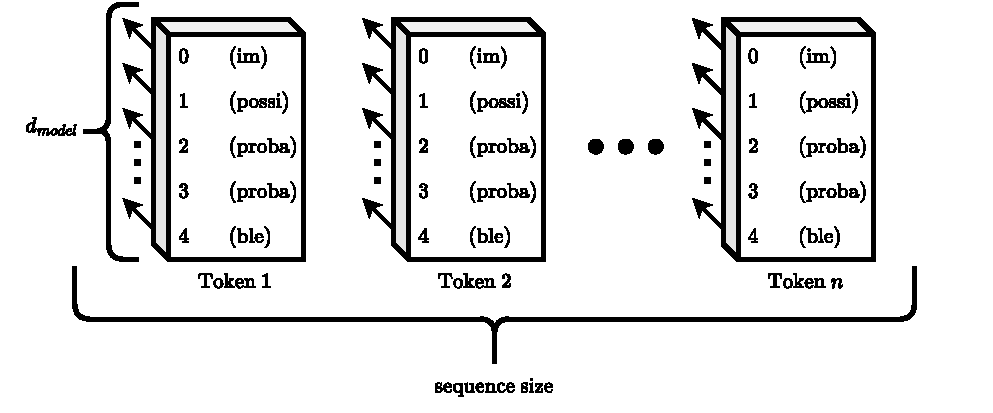
\includegraphics[width=0.85\textwidth]{embedding_layer.pdf}
  \caption{The embedding layer. Each rectangle represents one token slot of the embedding layer. Each slot outputs a feature vector of length $d_{model}$ that is fed into the following layer. The total amount of token slots is called sequence size. }
\label{fig:embed}
\end{figure}

%%% Word2Vec time
\section{Word Embedding}
Creating efficient word vector mappings was a challenge in the field of NLP for a long time until the invention of the Word2Vec model, which, for the first time, properly captured the semantic features of a word, which together represent the overall meaning of the word\,\cite{mikolov2013efficient}. For example, there might be a unit that is correlated with whether the token pertains to a living or unliving object or a value indicating its sex \ref{fig:clustering}.

Word2Vec uses two algorithms to train a shallow neural network for word-to-vector mapping\,\cite{mikolov2013efficient}:
\begin{itemize}
        \item \emph{Continuous Bag Of Words (CBOW)}: This algorithm predicts a hidden word based on the surrounding context without the knowledge of the word order.
        \item \emph{Skip-Gram}: This algorithm is exposed to one word and tries to predict its surrounding words.
\end{itemize}

%%% DIAGRAM clustering
\begin{figure}[]
  \centering
  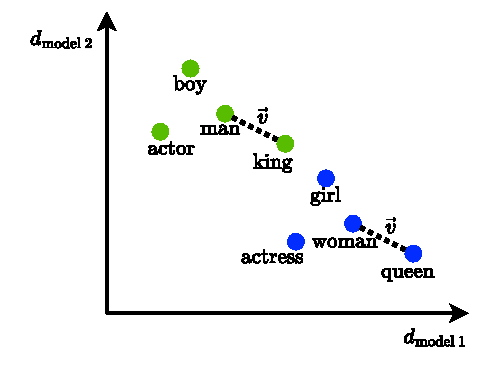
\includegraphics[width=0.6\textwidth]{clustering.pdf}
  \caption{Visualization of some well-trained token-to-feature mapping in two dimensions. Words related to men and women are clustered, respectively. Note that equivalent words in each cluster are spaced similarly. Such as the distance between man and king and woman and queen, which are both $\vec{v}$.}
  \label{fig:clustering}
\end{figure}

Interestingly, with a well-trained embedding mapping, it becomes possible to do arithmetic operations with the semantics of the tokens\,\cite{mikolov2013efficient}:

\begin{equation}
  \text{Embed}(\text{king}) - \text{Embed}(\text{man}) + \text{Embed}(\text{woman}) \approx \text{Embed}(\text{Queen})
\end{equation}

$\text{Embed}$ is a function of the embedding layer, transforming a word into a vector of features. In this example, the symbol ``$\approx$'' denotes a high degree of cosine similarity. Ideally, the difference between the left and right sides of the equation should be smaller than the difference between the right side and the embedding of any other token in the vocabulary\,\cite{mikolov2013efficient}.

By assigning an identification number to each token, the original text can be represented as a sequence of integers. Therefore, The input to the embedding layer can be a simple list of integers. The dimensionality of the embedding layer's output is called $d_{model}$ or sometimes \emph{feature size}.

The length of the sequence that the model can process at once is called the \emph{sequence size}. The number of available tokens is called \emph{vocabulary size}.

\section{Tokenization}
As was shown, tokenization is a powerful approach that enables us to feed textual data in and out of neural networks. However, in order to use tokenization, the vocabulary must be built first. It can have a significant impact on the performance of our model, so it is important to choose the right approach to generating it.

The most obvious solution might be to take the entire dictionary and make it our vocabulary. This approach is not ideal because the number of dictionary words is too large. During the training, less common words might not receive enough attention to develop their embedding mappings properly. This can be solved by removing less common words and representing their occurrences in the data with a generic \texttt{unknown} token, though this is obviously not a great solution either, as this results in the complete loss of meaning of those rare words.

Another obvious strategy would be to go for as minimal vocabulary as possible. Instead of including all possible words, all possible characters may be included. This approach even allows us to encode words from multiple languages and made-up words. However, with this approach, the advantages of vectorized representation are essentially forfeited because the neural network will have to learn to spell; this ultimately reduces learning potential.

In practice, vocabularies are usually created from the same datasets that will be used to train the neural network. There are two main approaches to generating vocabularies: \emph{top-down} and \emph{bottom-up}.

\subsection{Top-down}
With a top-down approach, a set of rules is defined and applied to the dataset, dissecting it into smaller and smaller pieces. Besides a simple conversion to token equivalents, the top-down approach often contains rules that change the text in some way, for example, expanding clitics\footnote{An example of expanding a clitic could be: $\text{don't} \rightarrow \text{do not}$}, removing certain punctuation, and so on. Top-down methods can often map multi-word entities to a single token, like \emph{New York}. One popular top-down approach is the Penn Treebank tokenization standard\,\cite{marcus-etal-1993-building}. In practice, regular expressions are often utilized to implement the rules, as they are deterministic and can be quite fast.

Some issues with the top-down approach arise when trying to parse languages that do not make use of spaces, such as Japanese and Chinese. For the Chinese, a character-based tokenization approach often yields superior results than other methods. In the case of Japanese, specialized word segmentation algorithms are needed.

\subsection{Bottom-up}
The bottom-up algorithm starts by examining the individual characters and applying rules to join multiple tokens to create one that covers more characters. Bottom-up tokenizers include tokens smaller than words, called sub-words. Among popular tokenization algorithms used today are unigram language modeling\,\cite{kudo-2018-subword} and byte-pair encoding\,\cite{sennrich-etal-2016-neural}.

\medskip

Byte-pair encoding was originally introduced as a compression algorithm\,\cite{bytePair1994}, but it was found to have great results as a tokenization algorithm.

The algorithm first adds all unique characters into the token vocabulary. Iteratively, it finds the most commonly occurring sequence of two tokens. It then adds a new token to the vocabulary representing the two tokens together and replaces all occurrences of these two tokens with the newly created one. This repeats until the quota on the total number of tokens is met. The algorithm doesn't cross spaces and, therefore, doesn't include any multi-word entities. Space itself is treated as a character that neighbors only the character to its left\,\cite{sennrich-etal-2016-neural}.

Provided that all possible tokens for a given task are included in the training set, the model avoids the use of the \texttt{unknown} token since, in the worst-case scenario of encountering a new word made up of unique parts, it can always be spelled using characters and sub-word tokens, but more common words and sub-words are still able to enjoy the benefits of semantic feature representation.

\medskip

During regular encoding, the tokenizer uses a greedy version of this algorithm, aiming for the longest token found in the vocabulary. Decoding is trivial, each token is mapped to its equivalent characters.

The idea behind bottom-up algorithms such as this one is that individual sub-word units ``morphemes'' will end up as tokens. For example, improbable consists of ``im'', which serves as a negation; ``prob'', the root which relates to the concept of probability; and ``able'', which is used to turn verbs into adjectives as shown in \ref{fig:embed}.

%% =============================================================
%%  _____                 __
%% |_   _| ___ _ _ _ __  / _| ___  _ __ _ __ ___   ___ _ __ ___
%%   | || '__/ _` | '_ \I |_ / _ \I '__| '_ ` _ \ / _ \ '__/ __|
%%   | || | | (_| | | | |  _| (_) | |  | | | | | |  __/ |  \__ \
%%   |_||_|  \__,_|_| |_|_|  \___/|_|  |_| |_| |_|\___|_|  |___/
%% =============================================================
\chapter{State of the Art}
\label{sec:llm}
This will go over \emph{Large Language Models (LLM)}, a technology utilizing neural networks with many layers to perform intelligent language processing. Starting with a short summary of the RNN-based models, followed by the introduction of attention, which is a core mechanism in Transformer-based models that recently revolutionized this field. 

Transformers are a family of Large Language Models based on the architecture of the original Transformer model created by Google in 2017. When first introduced, it outperformed all other contemporary machine-translation technologies by a significant margin. 

\medskip
% - attention
The invention of the transformer was preceded by the discovery of the attention mechanism described in\,\cite{bahdanau2016neural}. This paper introduced a novel technique for then-popular RNN-based architecture called \emph{Long Short-Term Memory LSTM}\,\cite{lstm1997} and its improved variant, the \emph{Gated recurrent unit GRU}\cite{gru2014} architecture. 

\medskip

Information in this chapter is primarily based on the book\,\cite{SpeechLanguageFeb2024} while information pertaining directly to the Transformer model is based on its foundational paper\,\cite{Transformer2023}.

\section{Recurrent Neural Networks}

Language processing with RNN-based neural networks suffers from poor context memory. Information stated earlier in the text is often forgotten, and too much weight is placed on recent parts of the sequence. In practice, this manifests as a drop-off in accuracy as the sequence size grows. This problem stems from the structure of the network itself; see \ref{fig:rnn}.

\begin{figure}[ht]
  \centering
  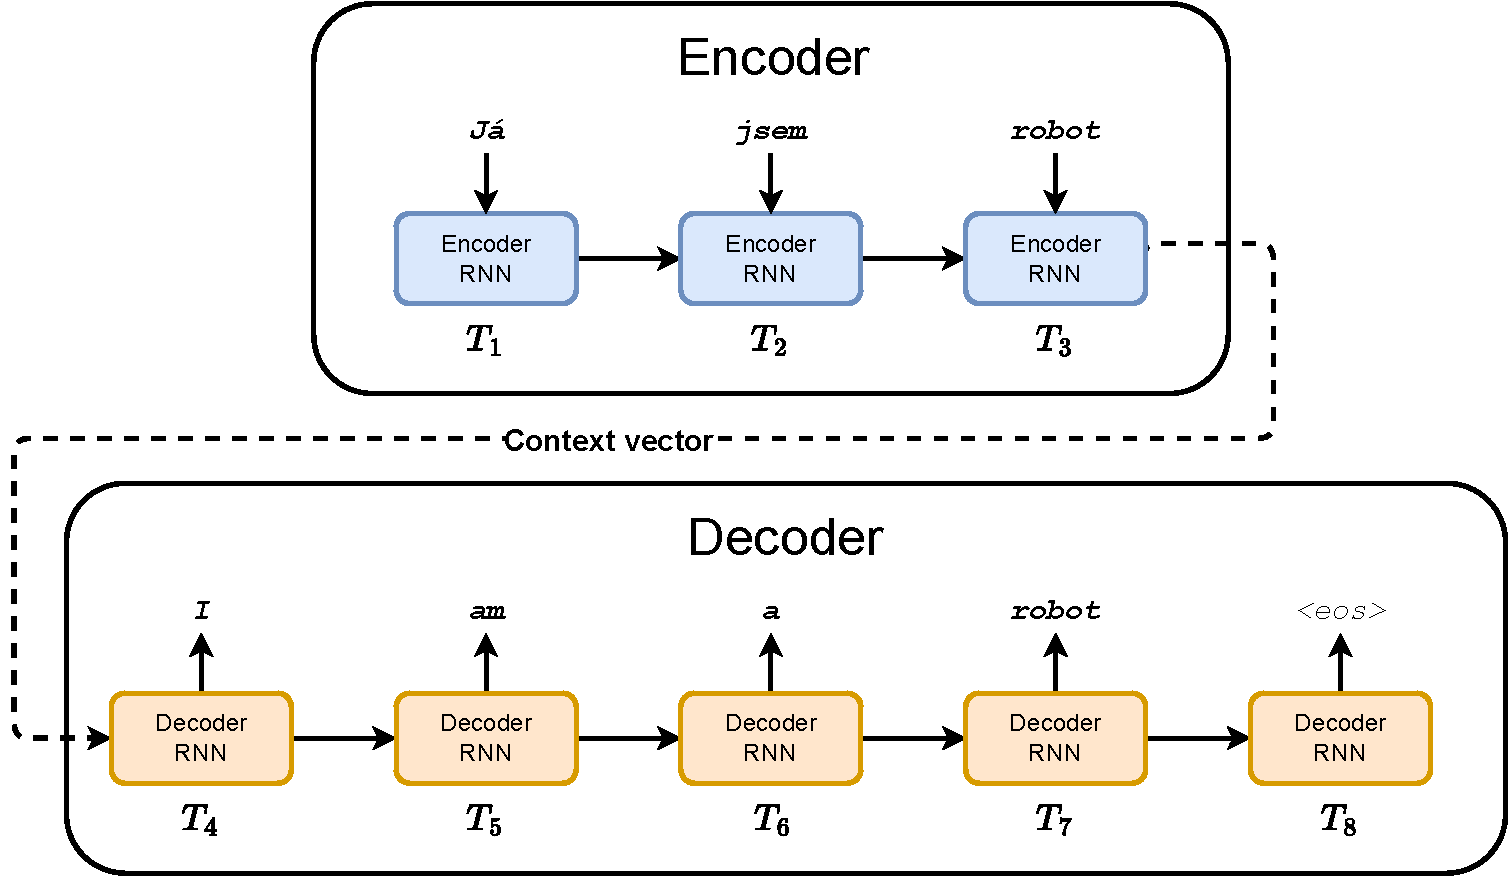
\includegraphics[width=0.66\textwidth]{encoder-decoder.pdf}
  \caption{
    Diagram of an RNN-based model performing a sequence-to-sequence translation. The model consists of two parts: an encoder and a decoder. Time steps are denoted as \(T_{n}\). Each input token is processed sequentially by the encoder RNN. The encoder receives the state from the previous time step and the current token as inputs.
    After all input tokens are processed, the encoder's final state is given to the decoder as an initial state.
  The decoder is an RNN for output generation; it repeatedly processes its previous state and outputs a token. The decoder iterates until the model generates an \texttt{end of sequence} (\texttt{<eos>}) token or some other condition is fulfilled.
  }
  \label{fig:rnn}
\end{figure}

Since the state is continually updated by newer inputs, information about older tokens gets overshadowed by information from later networks. LSTM has improved with this issue by introducing a gating mechanism\,\cite{lstm1997}, enabling the model to selectively retrain or forget information. Despite this advancement, this challenge was not fully overcome. The following paragraphs will describe the attention mechanism, which allows further improvements in context memorization.

\section{Attention}

Attention helps determine which parts of the input are relevant to the current state. Attention can be implemented in LSTM models by adding a third input to the decoder. First, all encoder states need to be saved. While decoding is underway, each of those states is concatenated with the decoder state and passed through a non-linear, fully connected layer. The results are scalar values representing the relevance scores of each input token in relation to the decoder state. The final context vector, which is the attention's output, is calculated as a sum of all encoder hidden layers scaled by their normalized attention scores. This kind of attention is called additive decoder attention\,\cite{sennrich-etal-2016-neural}.

\medskip

\section{The Transformer Model}
% - self-attention
The discovery of attention then led to an even larger breakthrough in the field of LLM when it was discovered that the properties of RNNs that made pre-attention language models so performant were now holding it back. Researchers at Google found that by complementing the attention mechanism with only a single-layered feed-forward network, the model was able to outperform competition in translation tasks without needing more complex components. The transformer was also computationally faster since it could be easily parallelized, thanks to the absence of feedback connections.

\begin{figure}[ht]
  \centering
  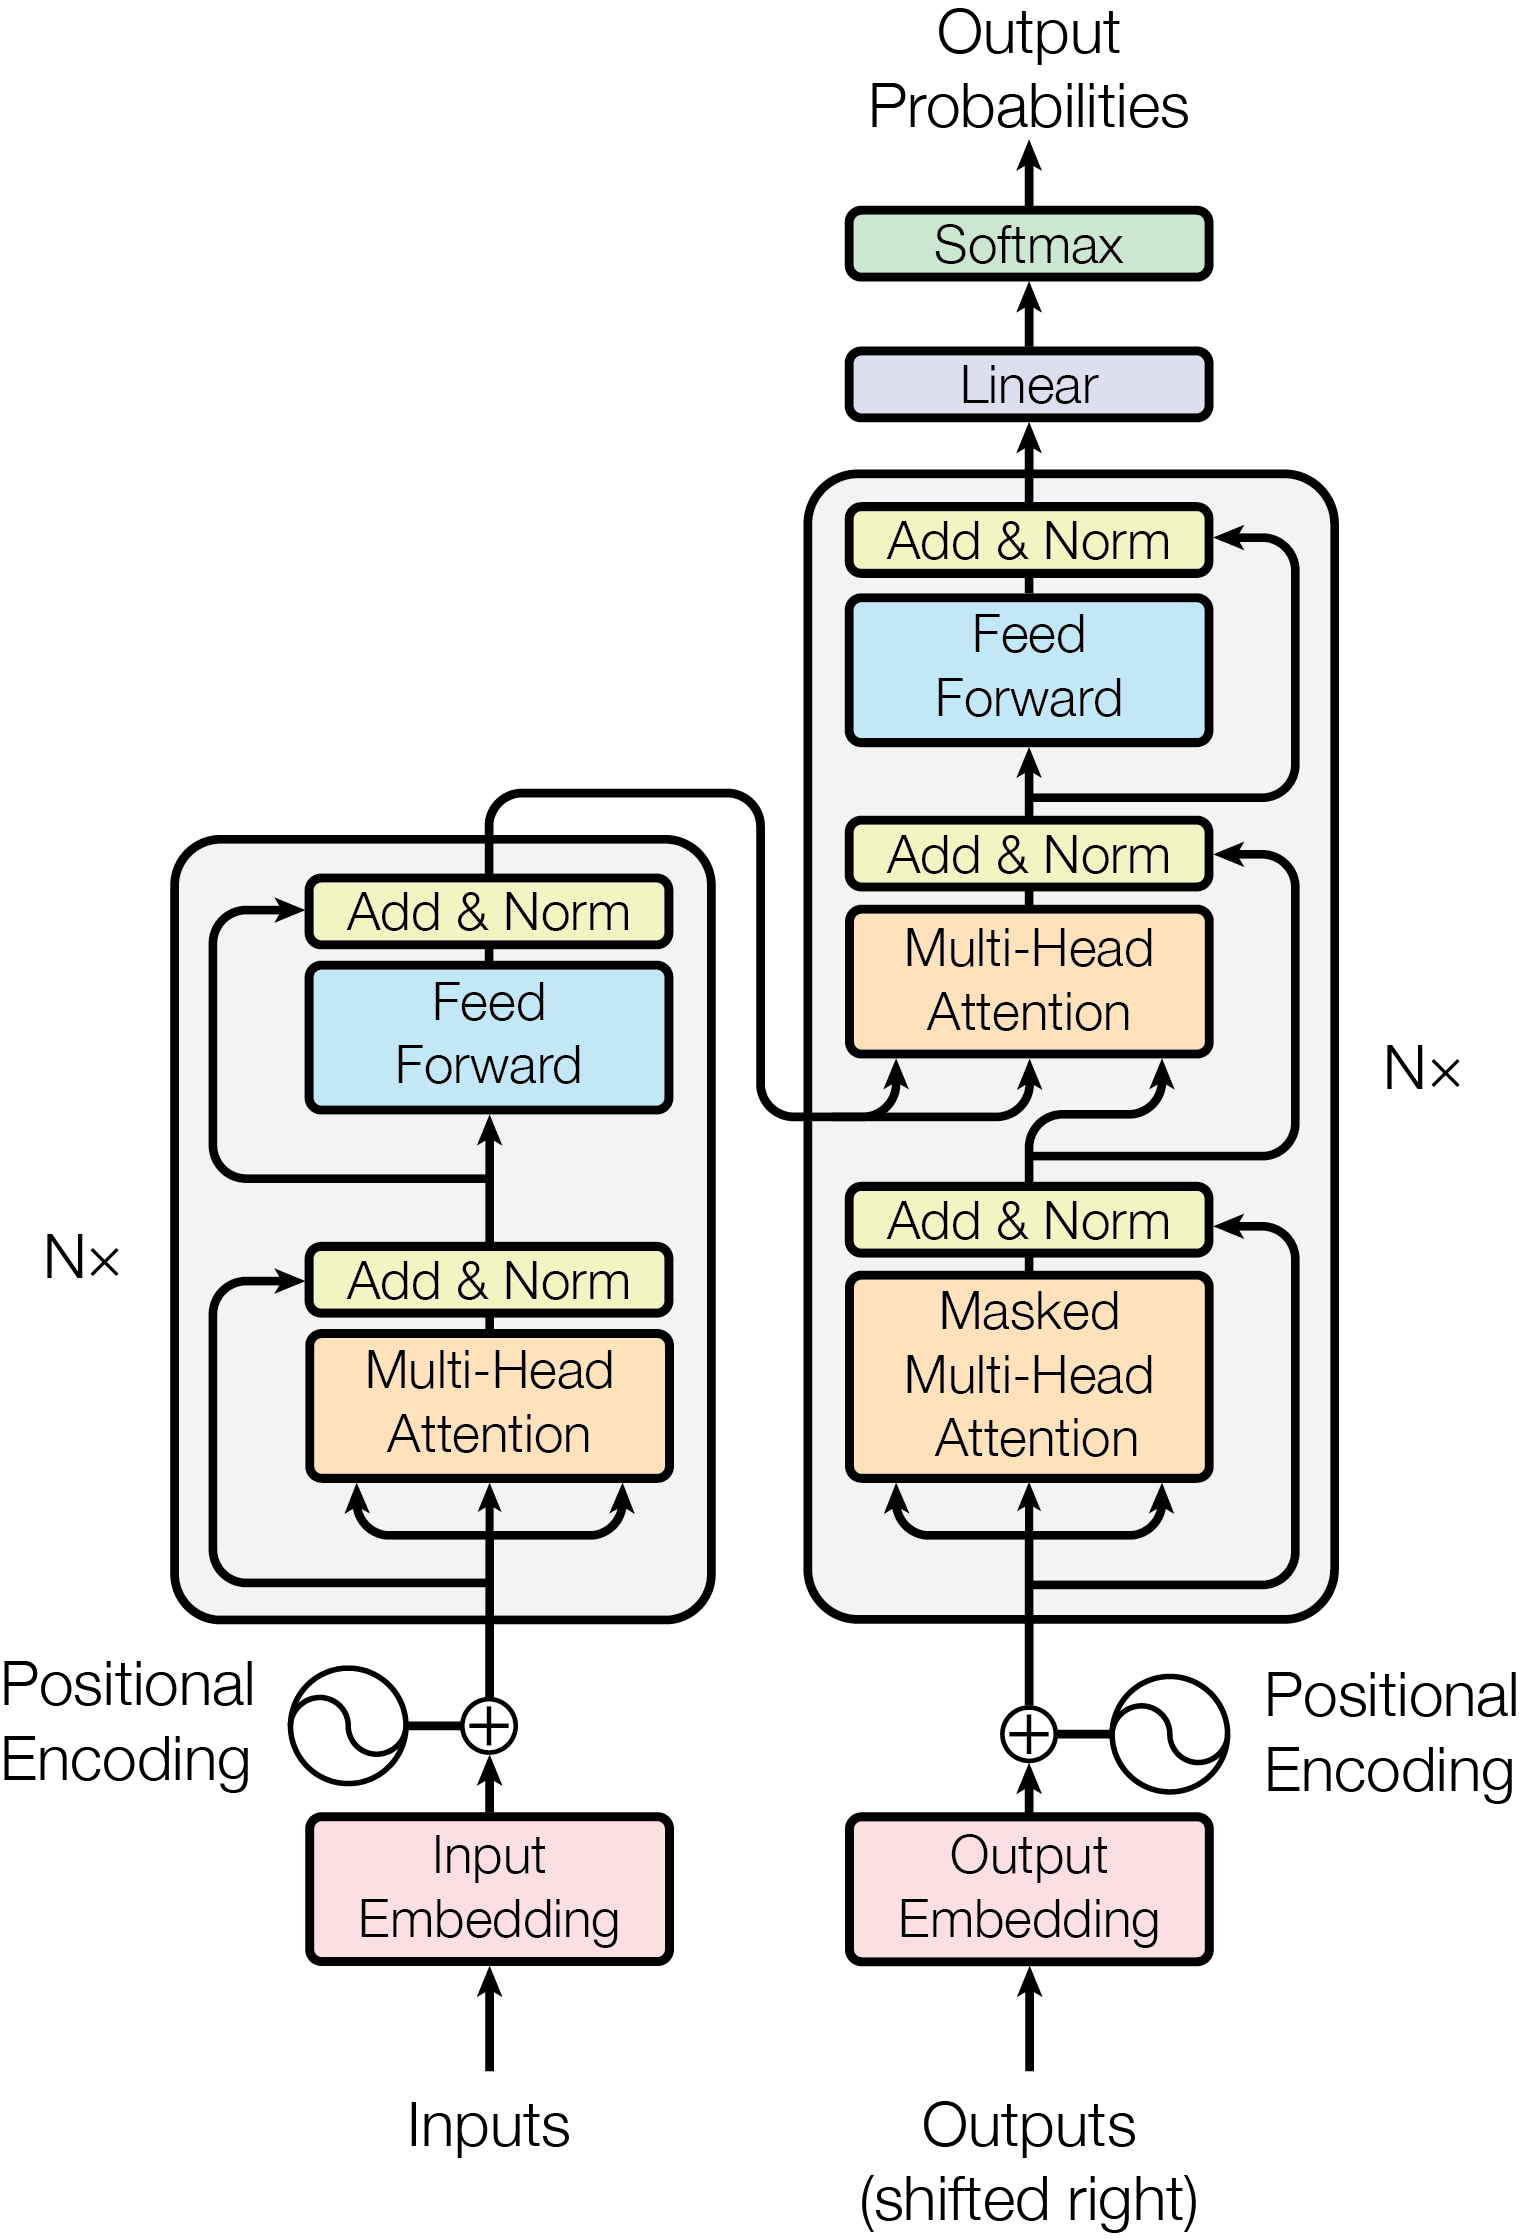
\includegraphics[width=0.53\textwidth]{ModalNet-21.png}
  \caption{The original transformer model. The encoder is depicted as the large block on the left and the decoder as the large block on the right. The encoder receives embedded input tokens with positional encodings, processes them, and gives its output to the decoder, which receives previously outputted tokens as input. The decoder's final hidden layer is used to determine the output token using the linear and softmax layers. This diagram was taken from Transformer's foundational paper\,\cite{Transformer2023}.}
  \label{fig:transformer}
\end{figure}

The transformer model uses its own variant of the attention mechanism, called \emph{multi-head self-attention} (figure \ref{fig:attention}). The attention formula itself is called \emph{scaled dot-product attention}. This method is called self-attention because it compares the input tokens with one another. The attention is calculated with the help of three intermediate matrices: \emph{Query $Q$, Key $K$ \emph{and} Value $V$}. Each is obtained by running the feature vector through a linear layer. The attention is calculated as follows:

\begin{equation}
  \text{Attention}(Q, K, V) = \text{softmax}(\frac{Q \cdot K^{T}}{\sqrt{d_{k}}})\cdot V
\end{equation}


$d_{k}$ is the dimensionality of $K$ and $Q$. In this case, the resulting attention is not a scalar but a vector of the same dimensions as the initial feature vector. This constitutes self-attention with a single head. When using multiple heads, the feature vectors are split so that every head processes an equal portion of the input. The output from the heads gets concatenated to restore its original dimensions.

\begin{figure}[ht]
  \centering
  \begin{subfigure}[t]{0.3\textwidth}
    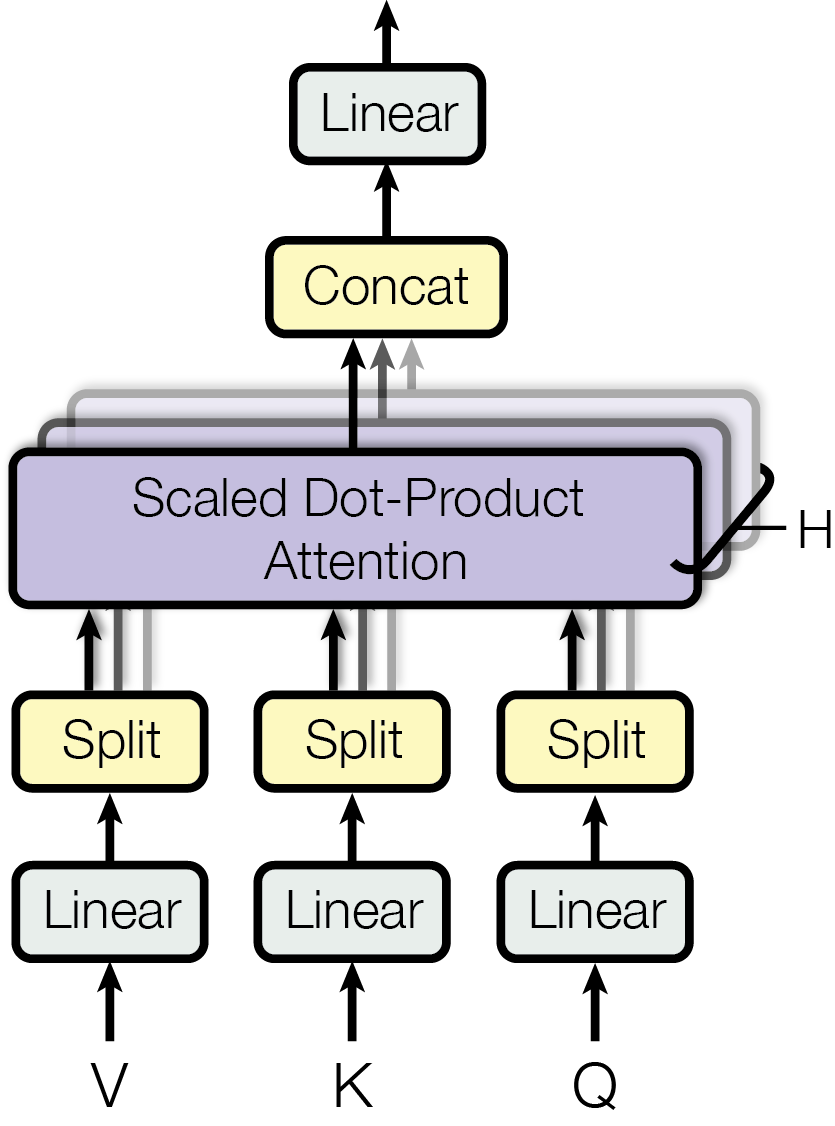
\includegraphics[width=\textwidth]{ModalNet-32.png}
    \label{fig:attention_a}
    \caption{}
  \end{subfigure}
  \hspace{3cm}
  \begin{subfigure}[t]{0.2\textwidth}
    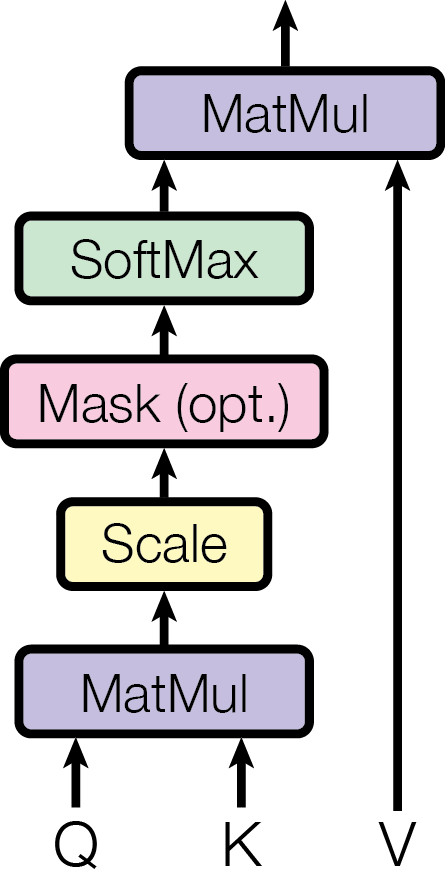
\includegraphics[width=\textwidth]{ModalNet-19.png}
    \label{fig:attention_b}
    \caption{}
  \end{subfigure}
  \caption{Attention block diagram. Image (a) is a diagram of multi-head self-attention, and image (b) is a diagram of \emph{scaled dot-product attention} calculation.}
  \label{fig:attention}
\end{figure}

\begin{figure}[ht]
  \centering
  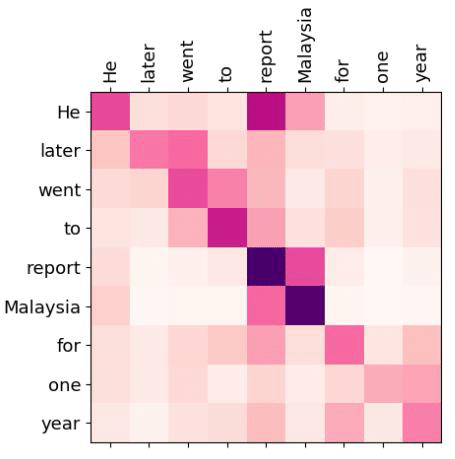
\includegraphics[width=0.40\textwidth]{attention-matrix.png}
  \caption{Example of a visualization of a self-attention matrix. Darker colors represent high activations. Note strong activation between semantically related tokens such as \emph{He} and \emph{report}. This figure was taken from\,\cite{attention-matrix}.}
  \label{fig:attention-matrix}
\end{figure}

One factor in which Transformers differ from earlier architectures is that the sequence size stays fixed after training. This is due to positional encoding, which is a mechanism that gives the transformer a sense of the order of the tokens. The position is encoded by adding a sine wave to even units of the vector and a cosine wave to the odd ones, with the frequency of the wave communicating the position. Like so:

\begin{equation}
PE(p,i) = g(p/10000^{{2i/d_{model}}})
\end{equation}

where $p$ is the token position, $i$ is the dimension in the vector and $g$ can be sine or cosine.

\medskip

% - encoder-decoder
The transformer uses an \emph{encoder-decoder} framework (figure \ref{fig:transformer}), also known as \emph{sequence-to-sequence (seq2seq)}, which was originally developed for the earlier RNN-based models. It splits the model into two parts: the first is called the \emph{encoder}, and the other is the \emph{decoder}. As the name suggests, the goal of this model is to transform one sequence of text into another. This architecture is useful for translations, where a sentence in one language is supplied as the input, and the sample sentence is translated into a different language as the label.

\subsection{Encoder}
% - encoder
The encoder receives the token embeddings with the positional encoding of the input sequence from the embedding layer. The encoder block typically repeats several times, six times in the original paper, but each time it uses different parameters.
\medskip
The encoder is centered around a residual pathway leading from the input to the output, providing a relatively unobfuscated path from the cost function to every trainable parameter to ensure strong gradients for all weights and biases. The residual pathway is first sampled by the \emph{Multi-head Attention}, which processes the feature vectors and then returns its output to the residual pathway. The addition is used to join processed outputs to the residual path and to prevent values from becoming too large; the residual pathway is then normalized.

The next in line to sample the pathway is a feed-forward network with one hidden layer. This layer typically has more neurons than input dimensions to capture more complex relationships. The output from the feed-forward then joins back with the residual pathway with addition and normalization, just like before.

The encoder's output captures the overall meaning of the input, often called the \emph{context}. It can either be paired with a decoder to perform sequence-to-sequence transformations, or it can be used for tasks such as sentiment analysis, classification, or searching.

\medskip

\subsection{Decoder}
% - decoder
The decoder runs interactively, each time generating a single token based on the context provided by an encoder.
A decoder block is not too different from an encoder; it is also built around a residual pathway that begins at an embedding layer, where, just like before, tokens are converted to their vector representation and enriched with positional encodings. However, this time, the network is fed a sequence of its own outputs from previous time steps. This provides the decoder with information about previous time steps. Before the first token is generated, the decoder is initialized with a special \texttt{beginning of sentence} token as input.
The output token of the decoder is obtained by passing the last activations from the decoder to a classification head, which is comprised of a linear layer and a softmax layer, where activation of each neuron represents a probability of a token.

The first on the residual pathway is multi-head attention. In this layer, it is crucial to mask out the token that is currently being predicted and all the ones that follow it to ensure that during training, the decoder learns to work only with tokens from the past. Then, the attention is calculated, and the result is merged back to the residual pathway like before.

% - cross-attention
Another operation on the residual pathway is a multi-head cross-attention. This is similar to self-attention, but instead of attending to itself, the decoder state attends to the encoder's output. Lastly, a decoder block ends with a feed-forward with one hidden layer.

Just like encoders, decoders can be used without an accompanying encoder. In this configuration, the cross-attention layer is omitted. Instead, the information about the input is supplied as initial tokens to the input; the decoder then generates new tokens to extend this sequence. This approach is quite popular. Among successful decoder-only models is OpenAI's GPT series.

% - Trénování transformerů
\subsection{Training Transformers}
Training transformers is the same as training any other neural network using gradient descent. The original Transformer uses the Adam (Adaptive moment estimation) optimizer, which is very popular with other Transformer-based model\footnote{Adam is used by BERT\,\cite{devlin2019bert}, GPT\,\cite{gpt32020} and many others.}. The Adam optimizer enhances regular gradient descent by dynamically adjusting the learning rate of each individual weight and bias based on two factors: The momentum of the gradient and the amount of fluctuation of the gradient\,\cite{kingma2017adam}.

A common technique to prevent overfitting is not using a gradient from a single inference but adding gradients from a batch of samples together. The batch gradient is divided by the number of samples in a batch so that the effective learning rate stays the same. Thanks to batching, the gradient is smoother and includes less sample-specific information. It can also be more performance efficient as the calculations of different samples can be done in parallel\,\cite{DeepLearning2016}.

If the input doesn't match the maximum input size exactly, it is necessary to fill the capacity with a special \texttt{padding} token, which is ignored during attention calculations.

% Pretraining
Modern LLMs have anywhere between hundreds of millions\footnote{Bart Base has 140 million parameters\,\cite{bart-2020}.} and billions\footnote{GPT-3 has over 175 billion parameters\,\cite{gpt32020} .} of parameters. Therefore, training them takes a considerable amount of money. Because of this, models are often trained in two phases. First, on general information relevant to a variety of tasks from a given domain, this technique is called \emph{pre-training}, and then they are exposed to a specific task, which is called \emph{finetuning}.

There are various strategies for pre-training an LLM, for example \emph{Denoising Autoencoder DAE} which works by corrupting the input data in some way\footnote{Corruption methods for DAE include: Token Masking, Chaining order of tokens, Removing tokens and others.} and comparing the output to the original text\,\cite{bart-2020}.

% Finetuning
After a model has been pre-trained using general text, it can be trained on a more specialized dataset to perform a specific task. This is called \emph{fine-tuning}. The fine-tuning process takes considerably less time and needs only a fraction of data than training from scratch would require.
A single pre-trained model can be used to fine-tune multiple models.
The inputs and outputs should be formatted the same way they will appear during deployment.

% - Decoding strategies

\subsection{Output decoding}
% sampling
The sampling method determines which token should be chosen as the output of the decoder. Notable ones include:
\begin{itemize}
        \item \emph{Greedy sampling}: The likeliest token is always greedily selected.
        \item \emph{Random sampling}: The output is chosen randomly based on the probability distribution outputted by the model.
        \item \emph{Top-k sampling}: The output is chosen from the $k$ likeliest tokens using random sampling. 
        \item \emph{Top-p sampling}: A pool that is made up of the most likely token up to a cumulative certainty of $p$ is randomly sampled.
\end{itemize}

% searching
Searching is another tactic for choosing the output:

\begin{itemize}
  \item \emph{Greedy search}: This is the simplest approach. At each step, only the likeliest token is chosen every time\,\cite{SpeechLanguageFeb2024}
        \item \emph{Beam search}: The algorithm keeps $n$ most probable sequences that it expands each time step. The output is the sequence with the highest cumulative probability.
\end{itemize}

\chapter{Tools and Technologies}
    
    The models have been trained using \emph{Torch}, a Free machine-learning library for Python that allows efficient tensor computing on the GPU. It also supports dynamic computational graph building, which is crucial for backpropagation. 
    
    Another important library used for the training is the \emph{Huggingface Transformers library}. It provides a unified framework for sharing models of different architectures while retraining a fine grip over the training process. Huggingface offers a library of Models of other architectures. Transformers library significantly streamlines the experimentation process of comparing different models in otherwise identical conditions, which is much more difficult while working with raw Torch models.

    Other Python libraries used in the project: \verb|SentencePiece|, \verb|toml|, \verb|accelerate|, \verb|astor|, \verb|peft|,  \verb|datasets|, \verb|bitsandbytes|, \verb|tqdm|, \verb|json|, \verb|nltk|, \verb|logging|, \verb|sacrebleu|.
    
    In order to train and evaluate the models, The Faculty's compute servers were heavily used, namely: \verb|pkcnot6|, \verb|pkcnot8|, \verb|athena19|, \verb|athena20|.
    
    \section{Sparse Attention Transformers} \label{led}
    % Teorie, důvod použití
    % Longformer, LED
    One of the biggest problems with training large language models is large memory size requirements. This factor often limits the sequence size and the number of parameters.

    The standard Transformer architecture suffers from \emph{quadratic memory complexity} in relation to the increase in sequence size, stemming from the nature of the attention mechanism\,\cite{child2019generating}. This results in very high memory usage, particularly during training where, when using the Adam optimizer, it is required to store one copy of the model, loss averages, loss momentum, and one or more gradients; each has the same memory size as the model. Fortunately, there are some approaches that can help lower memory consumption.

    \medskip
    
    The first one is sparse attention, a concept in which attention is only applied to a subset of the sequence, allowing for a lower memory footprint\,\cite{child2019generating}. Popular architectures include \emph{BigBird}\,\cite{zaheer2021big} and \emph{Longformer}\,\cite{beltagy2020longformer}. This paper makes extensive usage of the ladder. 

        Longformer achieves sparsity of the attention matrix by introducing two separate attention mechanisms, \emph{local attention} and \emph{global attention}.
        
        \begin{itemize}
            \item \emph{Local Attention} computed by a sliding window whose size is a fraction of the maximum sequence length. Local attention ensures that each token is attending to itself and a $w$ amount of tokens before and after. $w$ is the window size. See \ref{fig:sliding-window-attention}.
            
            \begin{figure}[H]
              \centering
              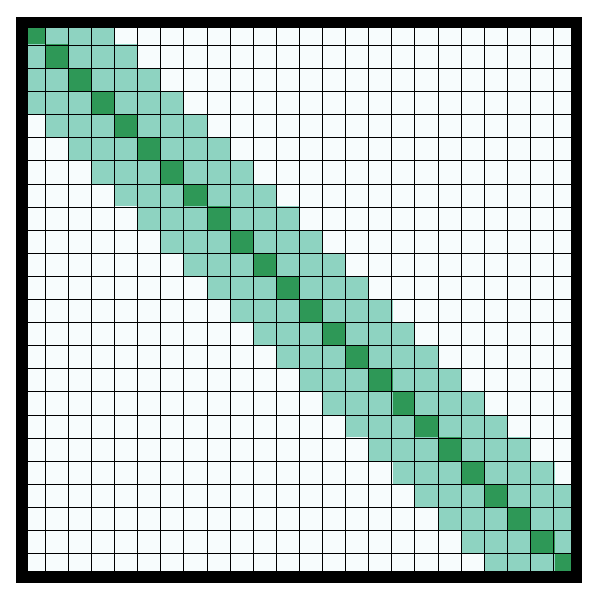
\includegraphics[width=0.4\textwidth]{obrazky-figures/fig-attn-window.pdf}
              \caption{Local attention diagram. The table represents attention between tokens; highlighted squares show that the row and column tokens are attending to each other. With traditional full attention, all squares would have been highlighted. The local attention window effectively reduces the number of attending tokens to a strip around the diagonal. In this particular case, the window size $w$ would be 3. Image taken from the Longformer paper\,\cite{beltagy2020longformer}.}
              \label{fig:sliding-window-attention}
            \end{figure}
            
            \item \emph{Global Attention} compliments local attention by enabling certain hand-picked tokens to attend to the whole input sequence. Allowing the model to better understand long inputs that contain important tokens that affect a larger part of the document. 
            \begin{figure}[H]
              \centering
              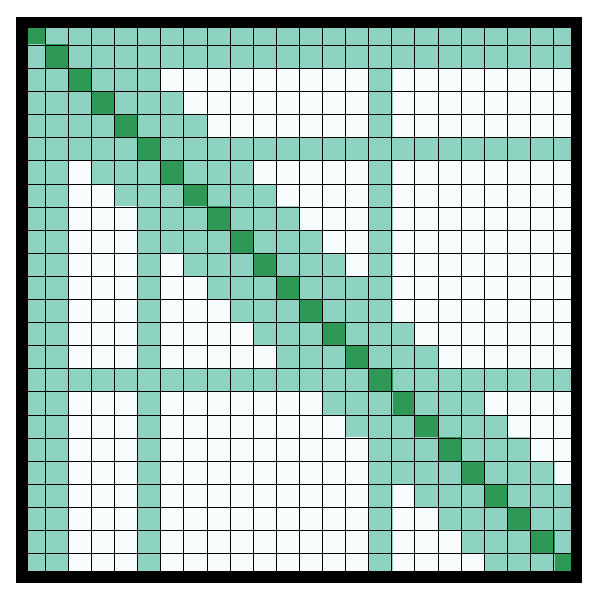
\includegraphics[width=0.4\textwidth]{obrazky-figures/fig-attn-combined.pdf}
              \caption{Local attention and Global attention together. The table represents attention between tokens; highlighted squares show that the row and column tokens are attending to each other. In addition to the diagonal strip, certain tokens are allowed to tend to the whole input like it is in full attention. Taken from the Longformer paper\,\cite{beltagy2020longformer}}
              \label{fig:global-attention}
            \end{figure}
        \end{itemize}

        The Longformer uses separate projection $QKV$ matrices for each Attention mechanism. Longformers architecture is, in a way, an extension of the RoBERTa\,\cite{liu2019roberta} model. In fact, it is possible to use a pre-trained RoBERTa model to \emph{initialize a Longformer}, in which case equivalent parameters are copied, and positional embeddings are extended via tiling. 
        
        The original Longformer model was developed as an encoder-only model, and some have even used it as an autoregressive model\,\cite{guo2023longcoder}. However, the standard version of Longformer \emph{does not support cross-attention}, so a separate model was developed for the purposes of sequence-to-sequence generation.

        \emph{Longformer Encoder-Decoder (LED)} is a sparse attention model that includes both an encoder and a decoder. Similarly to the original Longformer, it is extending a well-known model architecture, in this case, \emph{BART}\,\cite{bart-2020}, and may also be initialized with BART weights.

        \medskip

        This project extensively uses LED models, particularly those initialized with weights and biases of the \emph{PLBART model}\,\cite{ahmad2021unified}, a model trained on natural language and programming language. Thanks to the LED model, CodeImprove uses sequences of up to 2048 tokens despite the fact that PLBART only supports 512. In particular, the model was trained on natural language as well as Python and Java.

    \section{Quantized Low Rank adaptation} \label{qlora}
        Another approach is \emph{QLoRA or Quantized Low-Rank adaptation}\,\cite{dettmers2023qlora}. This technology allows the fine-tuning of very large language models with \emph{billions} of parameters on consumer-grade hardware by dramatically lowering the memory footprint of training.

        \medskip
        
        QLoRA is an improved version of \emph{LoRA (Low-Rank Adaptation)}. 
        
        As described in\,\cite{hu2021lora}, LoRA works by injecting additional parameters known as low-rank adapters into a pre-trained model and solely training those during fine-tuning, see \ref{fig:lora-diagram}. The rationale is that with a pre-trained model, you only need to alter the model a little bit to fine-tune it for a specific task, as most of the core knowledge was already obtained by the base model, and the inserted adapter parameters are simply steering the behavior in a certain direction. Of course, this means that this approach is only viable when fine-tuning.

        LoRA fine-tuning was found to have comparable results to full model fine-tuning and, in some cases, even surpassed it. In certain scenarios, LoRA might be achieving better results because it is not prone to catastrophic forgetting, a phenomenon in which the network quickly loses knowledge that is no longer being reinforced by the training data.

        %% LoRA diagram
        \begin{figure}[ht]
          \centering
          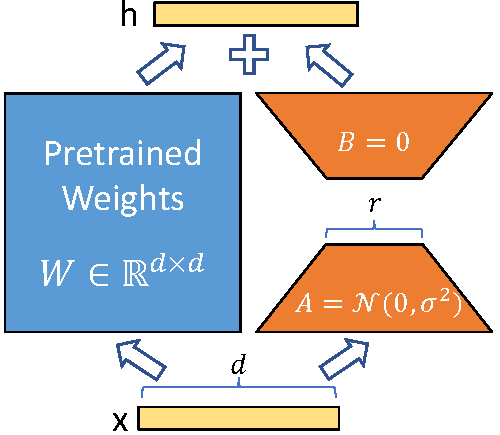
\includegraphics[width=0.5\textwidth]{obrazky-figures/LoRA.pdf}
          \caption{LoRA diagram. $x$ is the output of a previous layer, which is sampled not only by the original layer but also by the Lora adapter shown in orange. Each processes the $x$ in parallel, and the result is summed. $r$ is the size of the LoRA matrix. Figure taken from\,\cite{hu2021lora}.}
          \label{fig:lora-diagram}
        \end{figure}

        However, LoRA becomes even more useful when used alongside quantization. QLoRA is a recently introduced approach to LoRA that reduces parameter sizes to as little as 4 bits per floating-point number. This significantly increases training efficiency compared to the usual 16—or even 32-bit floats.

        To achieve this, QLoRA introduced in\,\cite{June2023qlora} presents a novel data type called \emph{4-bit NormalFloat}. As a 4-bit number, it can hold only 16 distinct states. Each of these states is assigned a value based on the distribution of values in model parameters, as shown in figure \ref{fig:qlora-distribution}. Usually, values of parameters form a normal distribution centered around zero. Parts of the spectrum with values that appear more often have smaller partitions than less populated parts.

        % Quant distribution diagram.
        \begin{figure}[H]
          \centering
          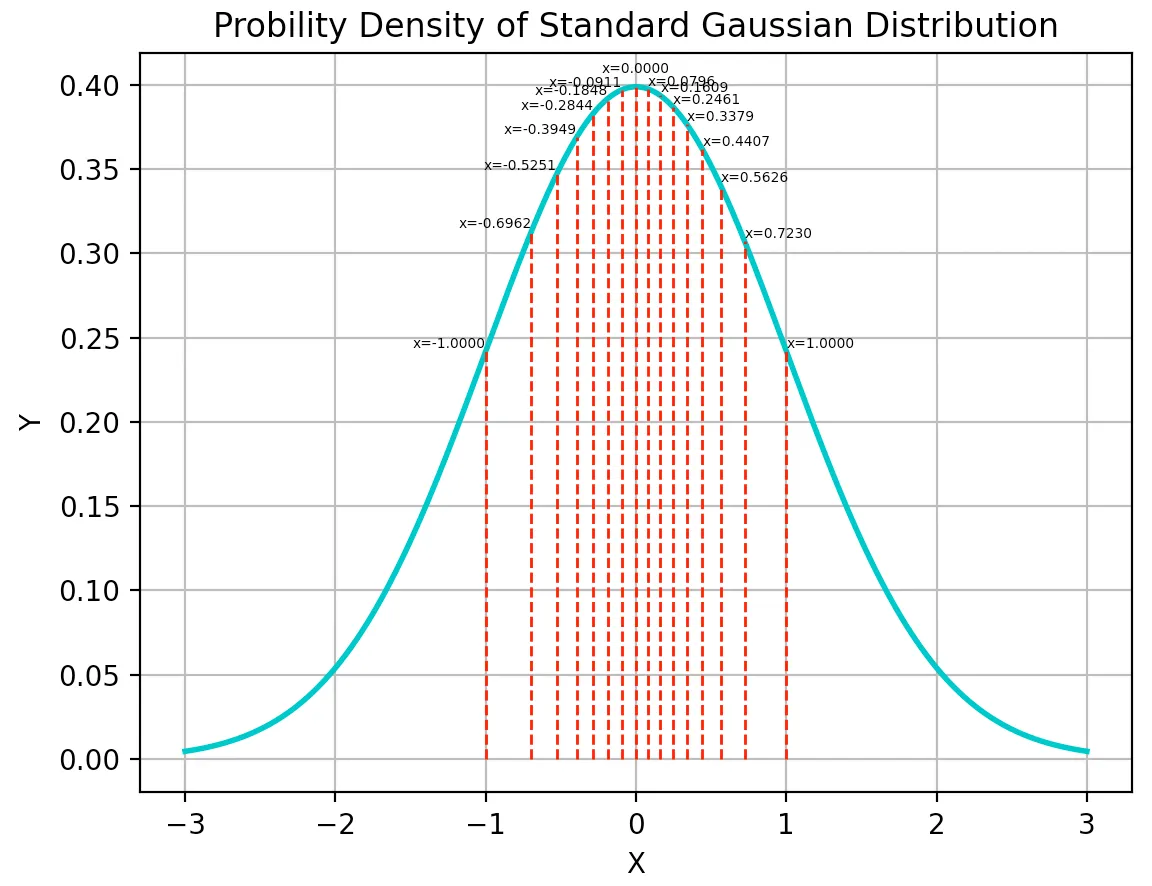
\includegraphics[width=0.8\textwidth]{obrazky-figures/qlora-normal-distribution.png}
          \caption{Example of some distribution of a 4-bit NormalFloat. The distribution of parameter values is in cyan, and the chosen values are in orange. Image taken from\,\cite{June2023qlora}.}
          \label{fig:qlora-distribution}
        \end{figure}
        
        During training, the original weights of the model are kept in their 4-bit form, and adapter weights are used in their 16-bit form, which saves a relatively large amount of memory. During inference, the entire model can be represented with just 4 bits per parameter.

\section{Used Datasets}
    Datasets are an important part of machine learning as their quality can bind the performance of the resulting model. This project makes use of two datasets for training.
    
    \subsection{Error Correction}
        In order to train the error correction module, a custom dataset was assembled from publicly available Freely licensed Python repositories, all of them publicly available on GitHub\footnote{GitHub: \url{https://github.com}}.
        
        Data was extracted from these repositories by first cloning their entire history and then searching commit messages using regular expressions for various iterations of the word \emph{fix}.
        
        A bug fix commit was accepted into the dataset if it contained only one hunk and changed two lines of code or fewer. The changes also had to be contained inside a single function or method body. 
        
        A snippet of the function before the patch, along with the title of the commit message, is used as the input, and the post-patch function is used as the label.
        
        Despite only accepting files ending in \texttt{.py}, it was crucial to conduct additional syntax checks, as many projects have long histories that extend back to Python 2.
        
        \medskip
        
        During this process, it could be observed that large, well-known projects contributed disproportionately more fixes than smaller projects, even if those smaller projects had a long history. This is likely due to the stricter committing etiquette that larger projects enforce, resulting in more concise and atomic commits, which fit the filtering criteria.
        
        Out of the total \emph{1213} repositories, \emph{only 565} contained commits that fulfilled the criteria. The total amount of samples is 16576.
        
        \medskip 
        
        In the pursuit of a larger sample size, the custom dataset is combined with PyTraceBugs\,\cite{pytracebugs}, which focuses on collecting tracebacks and related patches from GitHub issues. The dataset also offers before and after patches of Python functions. As a form of annotation of the samples, the dataset also includes information about the error message the faulty code produced when it crashed.
        
    \subsection{Comments and Rename}

        In order to train the two remaining modules, the \emph{CodeXGLUE code to text dataset}\,\cite{codexglue} was chosen. The main role this dataset fulfills is providing a large base of diverse Python code. The dataset is further reformatted to fit the requirements of both tasks.
    
\chapter{System Design}
    The past few years have seen a sharp influx of machine learning powered tools. Today, there are a plethora of products promising to help programmers with writing code. Among the most popular are GitHub Copilot\footnote{GitHub Copilot: \url{https://github.com/features/copilot}}, Tabnine\footnote{Tabnine: \url{https://www.tabnine.com/}} and Amazon CodeWhisperer\footnote{CodeWhisperer: \url{https://aws.amazon.com/codewhisperer/}}. Many developers also use ChatGPT\footnote{ChatGPT: \url{https://chat.openai.com/}}, which, despite not being marketed specifically towards developers, can handle code-related tasks rather well.
    
    Most of these tools are designed around generative models trained for instruction fulfillment and assistance. They require manual text prompt entry for each task (ChatGPT, GitHub Copilot, Tabnine, CodeWhisperer), where the programmer can specify a question or a task. Often, the AI will have access to the file that is currently open or at least to the highlighted code. Another commonly offered feature is predicting a string of tokens at the current cursor position (GitHub Copilot, Tabnine, CodeWhisperer).
    
    Despite recent technical developments, little has been done in terms of integrating more advanced AI tools into the editor's UI. This would be quite useful, especially for operations that need to be performed frequently and don't need any special details in the prompt. The CodeImprove extension offers such a service, utilizing more economical models for integrated refactoring aid.

    \section{Comment Suggestion Module} \label{comment_suggestion}
        One of the goals of CodeImprove is to enrich the source code with additional documentation in the form of comments. This is a quite complex task, so this work splits it into two parts:
        \begin{itemize}
            \item \emph{Comment detection:} The process of finding what parts of the code need additional documentation.
            \item \emph{Comment generation:} The process of generating the comments themselves.
        \end{itemize}
    
    
    \begin{figure}[H]
      \centering
      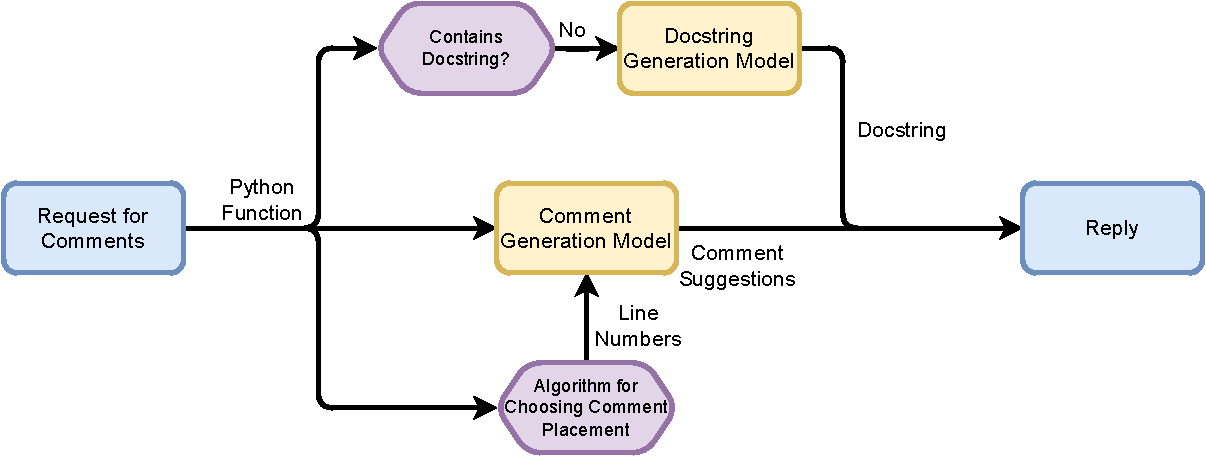
\includegraphics[width=1\textwidth]{obrazky-figures/comment-generation.pdf}
       \caption{Block diagram of the Comment Suggestion module.}
      \label{fig:comment-suggestion-led}
    \end{figure}
    
        \subsection{Comment Detection} \label{comment_detection}
            A docstring is the only kind of comment that has a set placement. The placement of every other comment is completely arbitrary and subject to personal preference.
            
            The initial solution for finding places in need of comments was using an LED model initialized from weights of the PLBart\,\cite{plbart2021} model, trained on the CodeXGLUE code-text dataset\,\cite{codexglue}. Though the dataset is formatted for training models on generating docstrings, it serves as a rich source of Python code that can be further modified to fit other purposes.
            
            In this case, Python's built-in modules \emph{AST} and \emph{tokenize} were leveraged to obtain information about lines that had a comment associated with them, either having a comment at the end of the line or a standalone comment on the line above.
            
            Input is created from the source by removing all of the comments and the docstring and annotating each line with its line number (listing \ref{lst:comment_source}. Global attention is placed on the (\texttt{end of sequence}) token and (\texttt{\_\_python\_\_}) token, and the label is constructed by joining the line numbers of the removed lines (listing \ref{lst:comment_source}).
            
            %% Example of data formatting running dataset_formators.py with global attention.
            \medskip
            \begin{figure}[H]
                \begin{lstlisting}[language=Python, caption={Sample Python code for showcasing dataset formatting. The function calculates $n$ elements of the Fibonacci sequence.}, label={lst:comment}]
    def fibonacci(n):
        """Calculates the Fibonacci sequence of length n."""
        # Initial sequence
        fib_sequence = [0, 1]
        while len(fib_sequence) < n:
            # Add two last numbers from the sequence together
            next_value = fib_sequence[-1] + fib_sequence[-2]
            fib_sequence.append(next_value)
        # Making sure we don't return more than the user has requested
        return fib_sequence[:n]
                \end{lstlisting}
            \end{figure}
            \begin{minipage}{.45\textwidth}
                \begin{lstlisting}[language=Python, caption={Code in listing \ref{lst:comment} formatted as an input for comment detection, italics denote global attention. \\ Note that the code has been ran through the PLBART's preprocessor function, which introduced \texttt{INDENT} and \texttt{DEDENT} tokens, as well as added spacing between tokens.}, label={lst:comment_source}]
    ^\textcolor{teal}{\$ 1 \$}^ def fib onacci ( n ) :
    ^\textcolor{teal}{\$ 2 \$}^ ^\textcolor{gray}{INDENT}^ fib_sequence = [ 0 , 1 ]
    ^\textcolor{teal}{\$ 3 \$}^ while len ( fib_sequence ) < n :
    ^\textcolor{teal}{\$ 4 \$}^ ^\textcolor{gray}{INDENT}^ next_value = fib_sequence [ - 1 ] + fib_sequence [ - 2 ]
    ^\textcolor{teal}{\$ 5 \$}^ fib_sequence . append ( next_value )
    ^\textcolor{teal}{\$ 6 \$}^ ^\textcolor{gray}{DEDENT}^ return fib_sequence [ : n ]
    ^\textcolor{teal}{\$ 7 \$}^
    ^\textcolor{gray}{</s> \textit{\_\_python\_\_}}^
                \end{lstlisting}
            \end{minipage}
            \hfill
            \begin{minipage}{.45\textwidth}
                \begin{lstlisting}[language=Python, caption={Code in listing \ref{lst:comment} formatted as a label.}]
    ^\textcolor{gray}{\_\_en\_XX\_\_}^ 2 4 6
                \end{lstlisting}
            \end{minipage}
            
            After training, the model's results appeared too noisy, primarily generating randomly looking lists of lines. It is possible that instead of learning the intricacies of what makes code require a comment, it was learning average distributions of comments.
            
            \medskip
            
            To get better results, the model was replaced by an algorithm that analyzes the syntax of the code and, through different criteria, chooses places for comment insertion. The heuristic evaluates a line as needing a comment if it contains more than 12 instances of unique identifiers, numbers, or operators in total, if the line was separated by the programmer from the line above by a blank line, or if the line contains one of the following branching control structures: \texttt{for}, \texttt{while}, \texttt{if}, \texttt{try}, \texttt{except}.
            
        \subsection{Comment Generation}
            CodeImprove differentiates between two kinds of comments: a regular hash-symbol (\texttt{\#}) comment, which describes lines that immediately follow it, and docstrings, which are multi-line string literals written at the start of a function or a method block and encapsulate information about the function, docstrings commonly describe what the function does, what each parameter is used for, and what its return value is; docstrings also often include code that showcases how to use the function.
            
            Docstring and comment generation are each handled by a separate model, though they are both trained on the same CodeXGLUE\,\cite{codexglue} code-text dataset as was the abandoned comment detection model; they also fine-tune the LED PLBart model. 
            
            \medskip
            
            When the dataset is loaded, every comment is either removed from the source (80\,\% probability) or kept (20\,\% probability). A sample for training and evaluation is created from each of the deleted comments. Each of these samples shares the same input, that being the source with the comments taken out, with one small change, the location of each comment is marked with \texttt{\$n\$}, where \texttt{\$n\$} is the particular line's number. The label is similarly formatted, starting with this special markup token followed by the content of this comment. The global attention is placed on the function declaration and also on the special markup sequence.

            
            In the case of docstrings, the marking in the input is placed at the very beginning and reads \texttt{\$ DOCSTR type \$}, where \texttt{type} identifies the formatting convention of the docstring and can either be \texttt{GO} for Google's convention\,\cite{GooglePythonStyleGuide}, \texttt{NP} for NumPy's convention\,\cite{NumPyStyleGuide} and \texttt{RE} for the reST convention\,\cite{SphinxPythonDomains}. In the training dataset, these different types of docstrings are classified using regular expressions.
            
            Pylint, TODO, and other kinds of non-descriptive comments are filtered out, along with commented source code, which is filtered by the presence of operators and is normally not included in regular comments.
            
            %% Example of encoded text
            \medskip
            \begin{minipage}{.45\textwidth}
                \begin{lstlisting}[language=Python, caption={Code in listing \ref{lst:comment} formatted as an input for comment generation to predict the docstring. Italics denote global attention. \\ Note that the code has been ran through the PLBART's preprocessor function, which introduced \texttt{INDENT} and \texttt{DEDENT} tokens, as well as added spacing between tokens.}]
    ^\textcolor{teal}{\textit{\$ DOCSTR NA \$}}^ ^\textit{\textcolor{blue}{def} fibonacci ( n ) :}^
    ^\textcolor{gray}{INDENT}^ fib_sequence = [ 0 , 1 ]
    while len ( fib_sequence ) < n :
    ^\textcolor{gray}{INDENT}^ next_value = fib_sequence [ - 1 ] + fib_sequence [ - 2 ]
    fib_sequence . append ( next_value )
    ^\textcolor{gray}{DEDENT}^ return fib_sequence [ : n ]
    ^\textcolor{gray}{</s> \textit{\_\_python\_\_}}
                \end{lstlisting}
            \end{minipage}
            \hfill
            \begin{minipage}{.45\textwidth}
                \begin{lstlisting}[language=Python, caption={Code in listing \ref{lst:comment} formatted as a label.}]
    ^\textcolor{gray}{\_\_en\_XX\_\_}^ ^\textcolor{teal}{\$ DOCSTR NA \$}^ Calculates the fibonacci sequence of length . ^\textcolor{gray}{</s>}^
                \end{lstlisting}
            \end{minipage}
    
            \medskip
    
            \begin{minipage}{.45\textwidth}
                \begin{lstlisting}[language=Python, caption={Another example of code in listing \ref{lst:comment} formatted as an input for comment generation to predict the comment on line 4. Italics denote global attention.}]
    ^\textit{\textcolor{blue}{def} fibonacci ( n ) :}^ 
    ^\textcolor{gray}{INDENT}^ fib_sequence = [ 0 , 1 ]
    while len ( fib_sequence ) < n :
    ^\textcolor{teal}{\textit{\$ 4 \$}}^ ^\textcolor{gray}{INDENT}^ next_value = fib_sequence [ - 1 ] + fib_sequence [ - 2 ]
    fib_sequence . append ( next_value )
    ^\textcolor{gray}{DEDENT}^ return fib_sequence [ : n ]
    ^\textcolor{gray}{</s>}^ ^\textit{\textcolor{gray}{\_\_python\_\_}}^
                \end{lstlisting}
            \end{minipage}
            \hfill
            \begin{minipage}{.45\textwidth}
                \begin{lstlisting}[language=Python, caption={Code in listing \ref{lst:comment} formatted as a label.}]
    ^\textcolor{gray}{\_\_en\_XX\_\_}^ ^\textcolor{teal}{\$ 4 \$}^ Add two last numbers from the sequence together ^\textcolor{gray}{</s>}^
                \end{lstlisting}
            \end{minipage}
    
    \section{Variable Name Suggestion Module}
        Among programmers, one can often hear joking remarks that coming up with names is the most difficult part of the job. CodeImprove aims to help with this issue by suggesting alternative names for variables in case the programmer feels like their creativity did not do a sufficient job.
        
        Because the variable's name is mostly rooted in the code that comes after its declaration, there is little to no point in suggesting code that is still unfinished.
        
        \medskip
        
        The renaming module is powered by a single LED model initialized with PLBART and is also trained on an altered version of the CodeXGLUE\,\cite{codexglue} code-text dataset. 
        
    \begin{figure}[H]
      \centering
      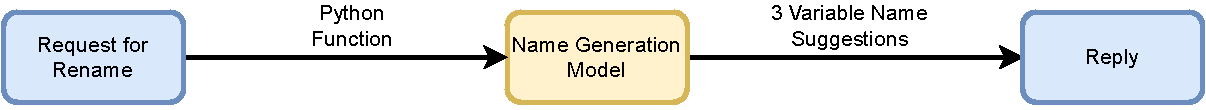
\includegraphics[width=1\textwidth]{obrazky-figures/name generation.pdf}
       \caption{Block diagram of the Variable Name suggestion module.}
      \label{fig:rename-led}
    \end{figure}
    
        Each sample from the dataset is parsed using the \texttt{AST} module. One variable identifier declared within the scope of the function is chosen, and all of its instances are masked out. The original name of the token is used as the label. Global attention is applied to the function definition and to all instances of the \texttt{mask} token.

        \medskip
        \begin{minipage}{.45\textwidth}
            \begin{lstlisting}[language=Python, caption={Example of code in listing \ref{lst:comment} formatted as an input for variable name generation, predicting a new name for \texttt{n}. Italics denote global attention.}]
def fibonacci ( ^\textcolor{teal}{\textit{<mask>}}^ ) :
^\textcolor{gray}{INDENT}^ fib_sequence = [ 0 , 1 ]
while len ( fib_sequence ) < ^\textcolor{teal}{\textit{<mask>}}^ : 
^\textcolor{gray}{INDENT}^ next_value = fib_sequence [ - 1 ] + fib_sequence [ - 2 ]
fib_sequence . append ( next_value )
^\textcolor{gray}{DEDENT}^ return fib_sequence [ : ^\textcolor{teal}{\textit{<mask>}}^ ]
^\textcolor{gray}{</s> \textit{\_\_python\_\_}}^
            \end{lstlisting}

        \end{minipage}
        \hfill
        \begin{minipage}{.45\textwidth}
            \begin{lstlisting}[language=Python, caption={Code in listing \ref{lst:comment} formatted as a label.}]
^\textcolor{gray}{\_\_python\_\_}^ count ^\textcolor{gray}{</s>}^
            \end{lstlisting}
        \end{minipage}
        
    \section{Error Correction Model with LED}
        The error correction feature of CodeImprove is meant to check the programmer's code for small errors and fix them. This module leverages a pair of LED PLBarts to first locate and then fix the errors. This approach is inspired by\,\cite{mashhadi2021applying}.
        
        Fixing errors can be very complex even for experienced programmers; in order to make this task achievable, the models focus on straightforward errors, which can be patched by changing two lines or less.
        
    \begin{figure}[H]
      \centering
      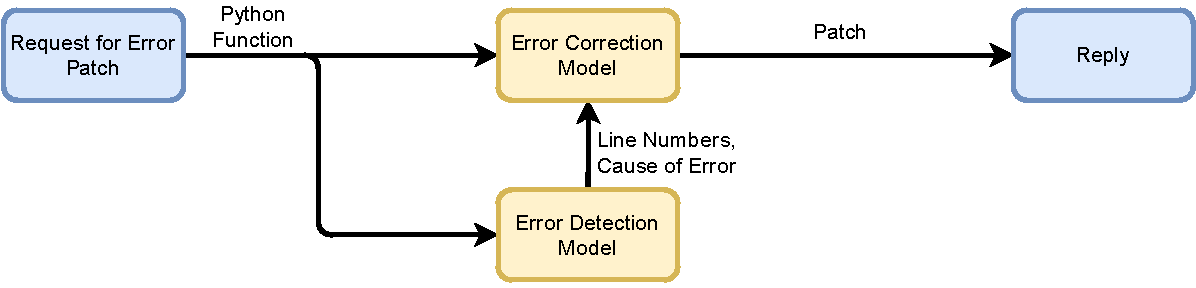
\includegraphics[width=1\textwidth]{obrazky-figures/error correction led.pdf}
       \caption{Block diagram of the Error Correction module using the LED model.}
      \label{fig:error-correction-led}
    \end{figure}
    
    \subsection{Error detection}
        The error detection module judges whether a given snippet contains errors and, if so, locates the lines on which it occurs.
        
        The input is annotated with line numbers enclosed in dollar signs, and the labels are a string of numbers that contain the error separated by spaces.
        
        Of course, not every snippet of code contains errors, and the model should be able to learn that. For this reason, the dataset is supplemented with examples of correct snippets taken from the stable code set of the PyTraceBugs dataset\,\cite{pytracebugs} in the ratio of 1:1.
        
        %%% Example of processed data
            \begin{lstlisting}[language=Python, label={lst:error}, caption={Example of a code snippet with an error. There should be \texttt{append} instead of \texttt{add} as highlighted in red.}]
def fibonacci(n):
    fib_sequence = [0, 1]
    while len(fib_sequence) < n:
        next_value = fib_sequence[-1] + fib_sequence[-2]
        fib_sequence.^\textcolor{purple}{add}^(next_value)
    return fib_sequence[: n]
            \end{lstlisting}
            
                \medskip
            \begin{lstlisting}[caption={Error description}]
Fixed bad method name\end{lstlisting}

        \begin{minipage}{.45\textwidth}
            \begin{lstlisting}[language=Python, caption={Example of code in listing \ref{lst:error} formatted as an input for error detection. Italics denote global attention.}]
^\textcolor{teal}{\$ 0 \$}^ def fibonacci ( n ) : 
^\textcolor{teal}{\$ 1 \$}^ ^\textcolor{gray}{INDENT}^ fib_sequence = [ 0 , 1 ] 
^\textcolor{teal}{\$ 2 \$}^ while len ( fib_sequence ) < n :
^\textcolor{teal}{\$ 3 \$}^ ^\textcolor{gray}{INDENT}^ next_value = fib_sequence [ - 1 ] + fib_sequence [ - 2 ]
^\textcolor{teal}{\$ 4 \$}^ fib_sequence . ^\textcolor{purple}{add}^ ( next\_value )
^\textcolor{teal}{\$ 5 \$}^ ^\textcolor{gray}{DEDENT}^ return fib_sequence [ : n ]
^\textcolor{gray}{</s> \textit{\_\_python\_\_}}^
            \end{lstlisting}
        \end{minipage}
        \hfill
        \begin{minipage}{.45\textwidth}
            \begin{lstlisting}[caption={Code in listing \ref{lst:error} formatted as a label for error detection.}]
^\textcolor{gray}{\_\_en\_XX\_\_}^ Fixed bad method name
5 ^\textcolor{gray}{</s>}^
            \end{lstlisting}
        \end{minipage}
        
    \subsection{Patch Generation}
    
        When it comes to generating patches, the model is trained with the pre-patch snippet as input, again annotated with line numbers. The output comprises a custom text difference notation along with an explanation of the error.
        
        The text difference format this module uses is quite simple. Each change note begins with the line number of the line being changed, followed by the new content of the line. If the line was deleted in the path, nothing follows the line number. This is different from a change to a blank line, as it would have contained a line feed. Insertion is represented by additional text after the line feed. It is theoretically possible to insert as many lines as we want.
        
        The goal behind creating this format was to free the model from having to recite the many lines of error-free code while remaining simple. 
        
        This functionality is powered by \emph{difflib}, which can smartly identify differences on the least possible amount of changes made. It outputs the traditional \texttt{diff} format, which is then transformed into this custom version.
        
        \begin{minipage}{.45\textwidth}
            \begin{lstlisting}[language=Python, caption={Example of code in listing \ref{lst:error} formatted as an input for error patching. Italics denote global attention.}]
^\textit{Fixed bad method name}^
^\textcolor{teal}{\$ 0 \$}^ def fibonacci ( n ) :
^\textcolor{teal}{\$ 1 \$}^ ^\textcolor{gray}{INDENT}^ fib_sequence = [ 0 , 1 ] 
^\textcolor{teal}{\$ 2 \$}^ while len ( fib_sequence ) < n : 
^\textcolor{teal}{\$ 3 \$}^ ^\textcolor{gray}{INDENT}^ next_value = fib_sequence [ - 1 ] + fib_sequence [ - 2 ]
^\textcolor{teal}{\$ 4 \$}^ fib_sequence . add ( next_value ) 
^\textcolor{teal}{\$ 5 \$}^ ^\textcolor{gray}{DEDENT}^ return fib_sequence [ : n ]
^\textcolor{gray}{</s> \textit{\_\_python\_\_}} 
            \end{lstlisting}
        \end{minipage}
        \hfill
        \begin{minipage}{.45\textwidth}
            \begin{lstlisting}[caption={Code in listing \ref{lst:error} formatted as a label for a patch.}]
^\textcolor{gray}{\_\_python\_\_}^ ^\textcolor{teal}{\$ 5 \$}^ fib_sequence . append ( next_value )
^\textcolor{gray}{</s>} \end{lstlisting}
        \end{minipage}
        
    \section{Error Correction Module with CodeWizard}
    Having observed the shortcomings of the LED variant of this module, it was decided to conduct another experiment with the suspicion that the reason for the poor performance of the previous one was due to a lack of neural complexity. WizardCoder\,\cite{luo2023wizardcoder} was selected as the new pre-trained model. It was chosen for its diverse range of size variants and relatively high performance in the lower billions\footnote{Benchmark scores can be viewed here: \url{https://huggingface.co/spaces/bigcode/bigcode-models-leaderboard}}.

    WizardCoder is a pre-trained autoregressive model, trained on fulfilling instructions using code and natural language, WizardCoder is trained on examples that were augmented in a process called \emph{Evol-Instruct}, which involves asking an already trained model to increase the difficulty of a sample from a dataset and then using the hardened samples to train a new model\,\cite{luo2023wizardcoder}. 
    
    This project uses an instruction fine-tuned variant of this model with \emph{one billion} parameters.
    
    The model checkpoints of WizardCoder have been recently unpublished for unclear reasons. However, the checkpoints are licensed as Free Software.
    
    This project utilizes QLoRA 4-bit quantization \ref{qlora} to reduce the training and inference costs of the model, which would have otherwise been too high. Using QLoRA training, the model becomes feasible even at the 2048 token limit on available hardware.
    
    An experiment was conducted with a diff-like output identical to the one used in the LED experiment (see formatting of input data listing \ref{lst:wizard-patch}) and a full code output (see formatting of input data listing \ref{lst:wizard-code}.)

  \begin{figure}[H]
  \begin{lstlisting}[caption={Prompt used to adapt WizardCoder to correct errors by generating patches.}, label={lst:wizard-patch}, numbers=none]
    Try to see if the following code has any errors. If not say \"No errors\" if it does explain the error and write a patch with the help of the line numbers.
    ### Code:
    <source code annotated with line numbers>
    ### Fixed Code:
   \end{lstlisting}
   
  \begin{lstlisting}[caption={Prompt used to adapt WizardCoder to correct errors by rewriting the code without the error.}, label={lst:wizard-code}, numbers=none]
    Try to see if the following code has any errors. Explain the error and write a fix it.
    ### Code:
    <source code>
    ### Fixed Code:
   \end{lstlisting}
  \end{figure}
    \begin{figure}[H]
      \centering
      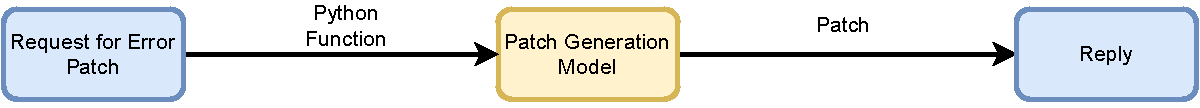
\includegraphics[width=1\textwidth]{obrazky-figures/error-correction-wizzrard.pdf}
       \caption{Block diagram of the Error Correction module using the Wizard model.}
      \label{fig:error-correction-wizzard}
    \end{figure}
%%%%%%%%%%%%%%%%%%%%%%%%%%%%%%%%%%%%%%%%%%%%%%%%%%%%%%%%%%%%%%
%% ###                                                        
%%  #  #    # #####  #      ###### #    # ###### #    # ##### 
%%  #  ##  ## #    # #      #      ##  ## #      ##   #   #   
%%  #  # ## # #    # #      #####  # ## # #####  # #  #   #   
%%  #  #    # #####  #      #      #    # #      #  # #   #   
%%  #  #    # #      #      #      #    # #      #   ##   #   
%% ### #    # #      ###### ###### #    # ###### #    #   #   
%%%%%%%%%%%%%%%%%%%%%%%%%%%%%%%%%%%%%%%%%%%%%%%%%%%%%%%%%%%%%%

\chapter{Implementation Details}
    The implementation of CodeImprove can be split into three parts. First, the training and experimentation software is implemented as a collection of Python and shell scripts. The server is also implemented in Python and uses some of the training infrastructure. Lastly, the client extension follows the standard format for Code extensions and is implemented in JavaScript.
    
    \section{Training}
    In the CodeImprove project, the training process itself is facilitated by \texttt{train.py}, which begins by parsing command line arguments using the \texttt{parse\_args} function from the \\ \texttt{my\_params} module. Then, the model loads a tokenizer with the assistance of the aforementioned Transformers library. 

    \subsection{Loading the Model}
    
        Next, based on a given \texttt{mode} command-line parameter, the script selected a proper data formatting function. This is done to accommodate the various kinds of models CodeImprove uses. The preprocessing functions themselves are defined in the \texttt{dataset\_formators} module. Then, the script loads the pre-trained model, which can be either an LED or a QLoRA model. 
        
        \medskip
        
        With QLoRA, the script also ensures that only the LoRA layers are used for training. Since the LED models used in this work are converted from pre-trained Bart models \ref{led}, we need to differentiate between layers that are initialized from scratch and layers that already contain relevant knowledge. 
        
        To dynamically find which layers are inherited from the Bart architecture, the script loads an additional Bart model and compares their state dictionaries. After that, the Bart model is unloaded from memory.
    
    \subsection{Loading Data}
    
        Then, the training data is loaded. The entry point for this operation is the \texttt{load\_data} function from the \texttt{my\_data} module. This function takes the tokenizer, the formatting function, and the parsed command line parameters and loads data entries from a \texttt{jsonl} file.
        
        \medskip
        
        The JSON Lines or \texttt{jsonl} format is a widely utilized file type for storing structured data in a compact and efficient manner. This format employs a simple but effective strategy where each line of the file represents a valid JSON object. This enables the data to be conveniently loaded and parsed in chunks or as a stream, allowing for more efficient processing and retrieval of information. 
        
        Each JSON entry is remapped into a native Python object for ease of use. Then, with the help of the formatting function, the data is filtered and tokenized to create the raw training data. This process creates the input and output token list and also a global attention mask, which is used with the LED models.
        
        The input and output tokens are first converted to IDs and padded to a uniform length, which is set as a command-line argument. \texttt{End of line} tokens are then appended. Finally, the script converts the data from lists to PyTorch tensors, which can be fed directly into the model.
        
        Additionally, attention masks are made for both input and labels by substituting the \texttt{padding} token with \texttt{False} and placing \texttt{True} everywhere else.
        
        This information is once again held in a custom object before being transformed into a dictionary with field names that conform to the standard naming for each respective element that the Transformer library expects. These dictionaries are returned in the form of a list, which finishes the data loading and preprocessing steps.
        
        \subsection{Training}
        The Transformers library offers a universal system for training models, which powers CodeImprove's training. First, a \texttt{TrainingArguments} object is created. This object stores the configuration of the training process with parameters such as batch size, the number of training epochs, and so on. It is initialized with the supplied command-line parameters.

        As stated earlier, the LED has two types of layers: those initialized with noise and those based on a pre-trained checkpoint of a BART model. We want to take a more aggressive approach during the training with the newly initialized layers and then with the pre-trained layers, as the gradients from the noisy layers could destroy the pre-trained knowledge.
        
        Because of this, a custom optimizer has been created. It accepts a learning rate for each of the two groups of layers. The reference code for this simplified optimizer was taken from one of the example scripts and modified to allow for the second learning rate.
        
        Layer freezing is another mechanism \texttt{train.py} uses to prevent the destruction of pre-trained knowledge. The pre-trained layers can be frozen for a configurable amount of training time. The eventual unfreezing is implemented via a \texttt{TrainerCallback}, and similarly, another call back is implemented that logs the values training statistics.
        
        Finally, the training begins, enclosed in a try-except that gracefully saves the model in case of an error or an interrupt signal.
        
        After the training, the model is saved to a file along with logged training information.

        \subsection{Training Configuration}

        For the LED models, the learning rate of $1 \times 10^{-5}$ for parameters inherited from PLBART and $3 \times 10^{-5}$ for newly initialized LED parameters proved to yield the best results. PLBART layers are also kept frozen for the duration of the first epoch. Warm-up steps, the number of steps during which the effective learning rate linearly moves from zero to the target learning rate, proved best when set in the lower thousands; for the final models, I have used the value of $1500$. A relatively high weight decay of $0.001$ worked well for preventing overfitting. The LED models took three iterations of the full CodeXGLUE code-to-text dataset to reach the point of underfitting.

    %%   ____ _ _            _   
    %%  / ___| (_) ___ _ __ | |_ 
    %% | |   | | |/ _ \ '_ \| __|
    %% | |___| | |  __/ | | | |_ 
    %%  \____|_|_|\___|_| |_|\__|
    \section{Client}
        In this case, the client is the Code extension. The extension focuses on providing quick and easy-to-use refactoring tools. 
        
        The extension makes use of Code's CodeLens API, which allows for rendering clickable text above chosen lines. The disadvantage of CodeLenses is that it creates spaces between the lines of code and moves the document. However, this only happens once when the extension is loaded, so the user should not feel major disturbances in their work.
        
        \medskip 
        
        CodeImprove uses these Code's \emph{DocumentSymbolProvider}, an API for generic programming language parsing, to obtain the list of all functions and methods in the document and uses it to display the options to scan the body of the code for Bugs and an option to generate new comments. 
        
        The extension also monitors changes in text selection, and when the user puts their cursor over variable declarations, it offers the name suggestion action.
        
        %% image of function and its CondeLense options
        \begin{figure}[ht!]
          \centering
          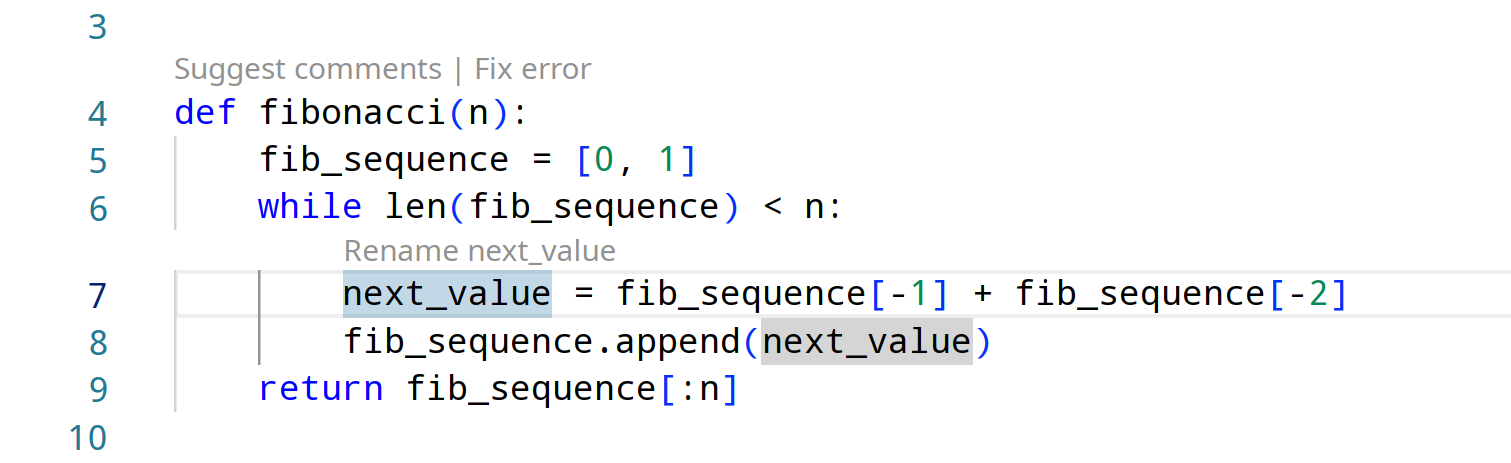
\includegraphics[width=\textwidth]{obrazky-figures/vscode-function.png}
          \caption{CodeLens options appearing around in a function, showing three clickable labels in total. The first two appear above the function definition, "Suggest comments" opens a panel with suggestions for extra code comments, and "Fix error" analyzes code for potential errors and offers a solution. The third appears on line 7 and reads, "Rename next\_value." Clicking it opens a variable name suggestion panel. This option is only shown because the user moved their text cursor over the variable name.}
          \label{fig:vscode_function}
        \end{figure}
        
        When the user clicks on any of these CodeLenses, a temporary side panel will open and display a loading screen while the extension sends a request to the server and, upon getting a response, displays it. The address and port of the server can be specified in the settings.
        
        \subsection{Comment Generation}
            The comment generation panel lets you change the docstring convention between no formatting, Google, NumPy, and reStructuredText. Underneath is a code view that displays how the function will look after the changes are applied. All comments stand alone on their own line. The docstring will be generated only if it was previously missing. Inserted lines appear highlighted in the code view. See figure \ref{fig:vscode_comments}.
        
        \begin{figure}[ht!]
          \centering
          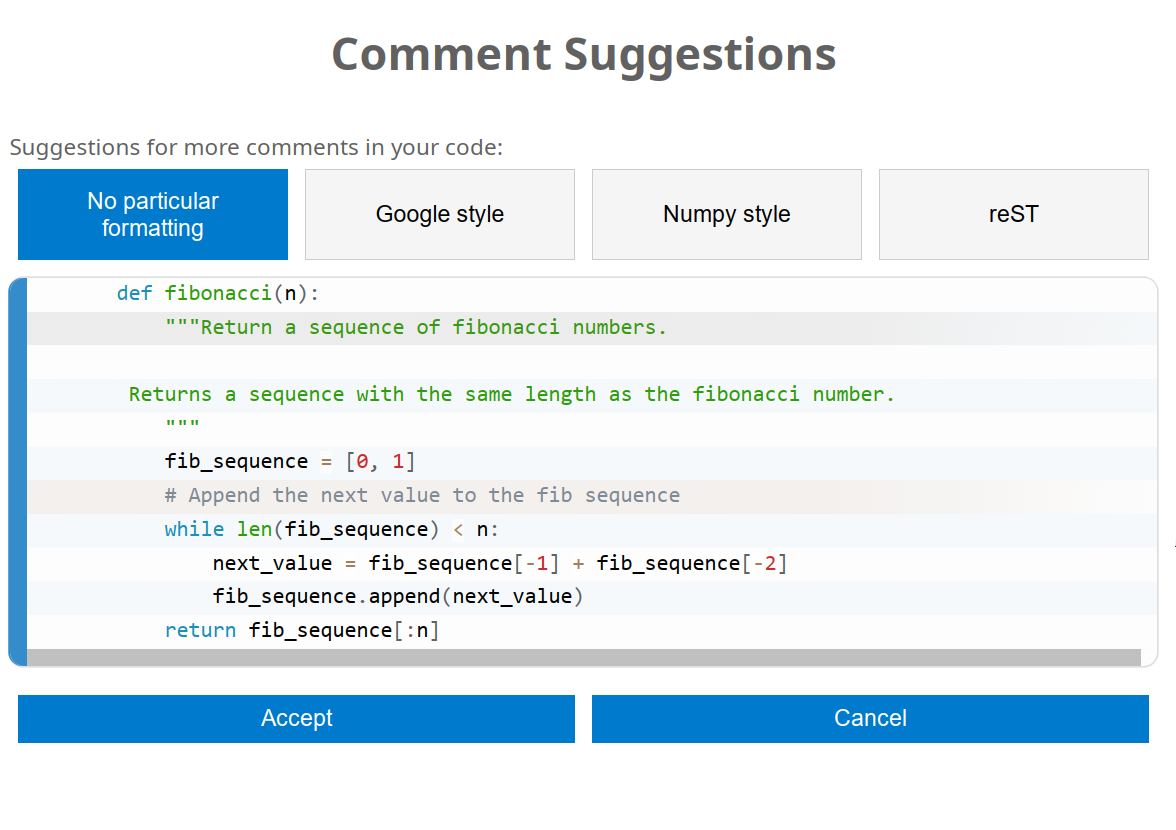
\includegraphics[width=0.8\textwidth]{obrazky-figures/CodeImprove-comment-screenshot.png}
          \caption{CodeImprove comment suggestion window. It is currently suggesting a new docstring and a comment above the while loop.}
          \label{fig:vscode_comments}
        \end{figure}
        
        \subsection{Error Correction}
            The error correction panel similarly uses a code view to display the suggested change, but this time, the data is displayed more like a traditional \emph{diff} view. Inserted lines are highlighted with a lighter color, and deleted lines with a darker color. Each line is annotated with a comment \texttt{New}, \texttt{Removed} for inversion and deletion, respectively, and \texttt{Before} and \texttt{After} for substituting the original line of text. These comments are only visible in this preview panel and won't be present in the code when the changes are applied. See figure \ref{fig:vscode_errors}.
        
        \begin{figure}[ht!]
          \centering
          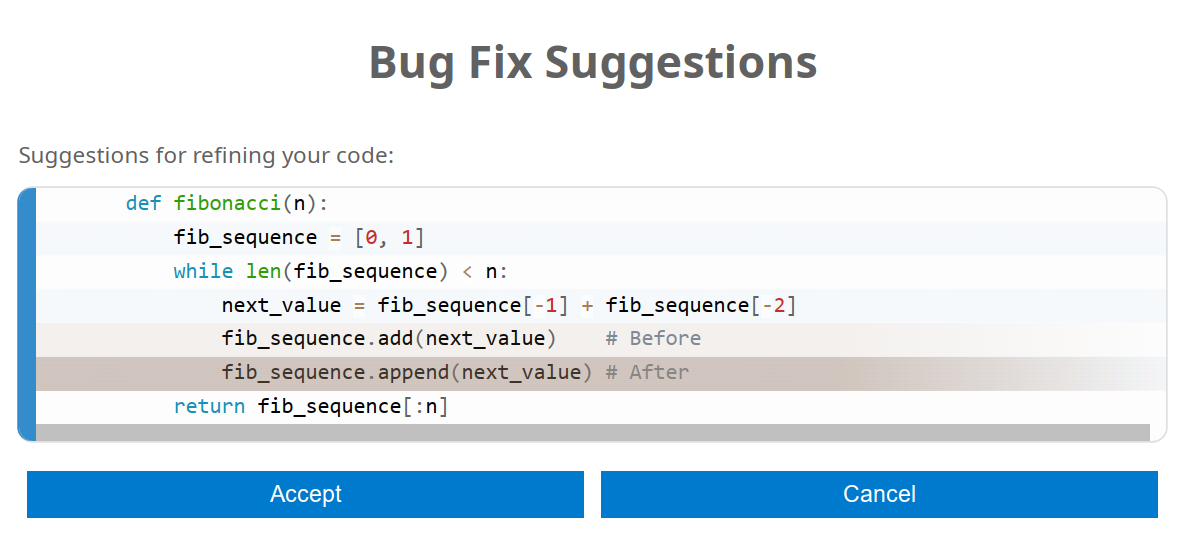
\includegraphics[width=0.85\textwidth]{obrazky-figures/codeimprove-bugfix.png}
          \caption{CodeImprove suggestion for error correction, changes are highlighted. Note that this suggestion was mocked.}
          \label{fig:vscode_errors}
        \end{figure}
        
        \subsection{Variable name suggestion}
            The renaming panel presents the user with three choices for a variable name, which the user selects by clicking on them. See figure \ref{fig:vscode_rename}.
        
        %% Rename screen
        \begin{figure}[ht!]
          \centering
          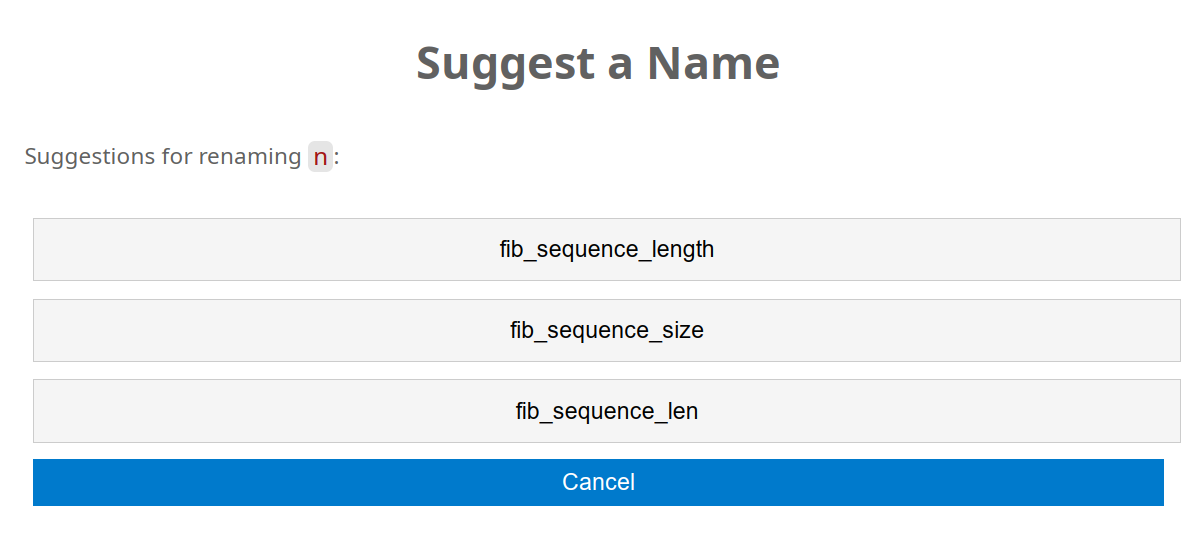
\includegraphics[width=0.85\textwidth]{obrazky-figures/codeimprove-rename.png}
          \caption{CodeImprove suggestion for an alternative variable name.}
          \label{fig:vscode_rename}
        \end{figure}
        
        \subsection{Scope of Functionality}
            CodeImprove operates only on functions and methods. Code that is not inside any of those code blocks cannot be evaluated; this decision stems from the Datasets and the ease of training. Functions provide a mostly closed-off window to code with a singular purpose; working with larger chunks of code would require high input length, introduce a lot of noise into the training, and require much larger models to evaluate.
        
            Likewise, code inside a function that is itself inside another function cannot be evaluated independently from its parent function, though this practice seems to be used only rarely in Python.
            
            The client receives instructions on what to change and composes the post-change code accordingly. The only exception is renaming, which has to have its post-change generated on the server side because Code does not expose any APIs for renaming identifiers, even though this functionality is available in the editor as a GUI feature. The only available option similar to this is \texttt{editor.action.rename}, which does not accept the new name and will only open the renaming dialog to the user. Hence, the choice of processing on the server came naturally after this, as Free JavaScript libraries do not offer the same level of quality when parsing Python code as Python's standard library.
            
    \section{Server}
        The server side is implemented in \texttt{server.py}, allowing users to run inferences on their code. It is controlled by a TOML configuration file, which specifies paths to each model and the configuration for running inference on them. The configuration file also includes a port on which the application communicates; by default, this is set to 8182.
        
        The server uses an event loop to wait for incoming requests. Upon a request, \texttt{server.py} will parse the request, select the appropriate model, and use the code formatting functions from \texttt{dataset\_formators} that are used for training, and in the case of LED models, it even calls the PLBART preprocessing function, to make sure that the data is presented to the model in a familiar form. 

        Responses are formatted into a JavaScript object and serialized as JSON before being sent back to the user.
        
\subsection{Communication}
    The client and the server exchange information via the HTTP protocol. The communication is completely stateless and uses the traditional request-response format. The client always initiates it via a \texttt{POST} request containing a JSON-encoded payload with structured information, such as the type of suggestion that is being requested and the snippet of the function code, see listing \ref{lst:request} for more details about the format of requests and listing \ref{lst:response} for responses.  
    
\capstartfalse
\begin{figure}[H]
  \begin{lstlisting}[caption={The request message data structure. \texttt{uuid} is meant for identification of the message, \texttt{requests} is a list of individual requests, identified with \texttt{id}, which is a serial number of the request, \texttt{snippet} contains the code snippet this request applies to and \texttt{tasks} is a list of task objects, each contains its task type in \texttt{task}, which is either "rename" for the suggestion alternative names to variables, \texttt{error} for fixing errors and \texttt{comment} for inserting additional comments. The field \texttt{symbol} is present only in \texttt{rename} tasks used to specify the name of the variable for renaming, and \texttt{style} is similarly only present in \texttt{comment} tasks and specifies the docstring preference.}, label={lst:request}, numbers=none]
Request Message {
    uuid: string
    requests: [
        {
            id: integer
            snippet: string
            tasks: [
                {
                    task: "rename" | "error" | "comment"
                    symbol: string (when task = "rename")
                    style: "NA" | "GO" | "NP" | "RE" (when task = "comment")
                }
            ]
        }
    ]
}\end{lstlisting}
  \centering
  \begin{lstlisting}[caption={The response message data structure. \texttt{uuid} matches the \texttt{uuid} of the request. \texttt{response} is a list of the individual responses. \texttt{id} and \texttt{task} together match up with their respective field in the request and serve to identify the response. \texttt{status} is meant to signify the result of the task. \texttt{result} contains the output of the task; for comment generation and error correction, this is a string; however, for the renaming task, this is a list where each element represents one rename suggestion and contains both the new name for the variable and the code snippet with the substituted name.}, label={lst:response}, numbers=none]
Response Message {
    uuid: string
    response: [
        {
            id: integer
            tasks: "rename" | "error" | "comment"
            status: "ok" | "error"
            result: string | list
            ]
        }
    ]
}
  \end{lstlisting}
\end{figure}

%%%%%%%%%%%%%%%%%%%%%%%%%%%%%%%
%% #######                      
%% #       #    #   ##   #      
%% #       #    #  #  #  #      
%% #####   #    # #    # #      
%% #       #    # ###### #      
%% #        #  #  #    # #      
%% #######   ##   #    # ######
%%%%%%%%%%%%%%%%%%%%%%%%%%%%%%%
\chapter{Evaluation and Results}
    Finally, CodeImprove's models need to be tested against the competition in order to judge their performance and usability.  GPT-3.5-turbo by OpenAI was chosen as the baseline for comparing performance since it is, from publicly available information, the closest model to the one used in GitHub copilot, or at least the closest that is publicly available.
    
    Each benchmark was computed from a thousand samples that CodeImprove has not seen during training; sadly, due to the nature of large-scale data collection OpenAI employs, it is impossible to verify that the same applies to the GPT-3.5-turbo model.
    
    \section{Assessment of Comment Generation}
        \subsection{\textsc{Bleu}}
        \textsc{Bleu} (Bilingual Evaluation Understudy) is a metric introduced by\,\cite{papineni-etal-2002-bleu}; it stands as one of the most prominent automated methods used for quantifying similarity between two pieces of text. \textsc{Bleu} evaluates the quality of machine-generated text by calculating the correspondence between it and a set of high-quality reference outputs. \textsc{Bleu} was originally developed to track the performance of translators, but it will serve us well when rating the similarity of a reference comment to one generated by our system.
        
        The goal of \textsc{Bleu} is to quantify similarity while allowing for changed word order or a partially different choice of words. Despite being based on a simple algorithm, \textsc{Bleu} was found to rate translations similarly to human reviewers.
        
        At its core, \textsc{Bleu} works by counting how many correct words (unigrams) from the prediction appear in the reference output, divided by the number of words in the prediction. The presence of a word only counts up to the number of occurrences of that particular word in the reference output. 
        The same is also done with sequences of two words (bigrams), three words (trigrams), and four words (guadgrams). The longer the measured sequence is, the lower the score will be in practice. To balance this, the scores are averaged with a geometric mean.
        
        Lastly, \textsc{Bleu} penalizes sentences that are shorter than the shortest reference translation with multiplayer.
    
        \begin{equation}
            BP = 
            \begin{cases} 
                1 & \text{if } c > r \\
                e^{(1-r/c)} & \text{if } c \leq r 
            \end{cases}
        \end{equation}
        Where $c$ is the number of words in the candidate, and $r$ is the number of words in the reference. 
        
        The full equation is a s follows:
        \begin{equation}
            \text{\textsc{Bleu}} = BP \times \exp\left(\sum_{n=1}^{N} w_n \log p_n\right)
        \end{equation}
        Where BP is the brevity penalty, $ p_n$ is the number of n-grams from the prediction that matches the reference. $w_n$ are weights assigned to each n-gram; typically,y these are 1/n. N is the size of the largest n-gram 
            
    \subsection{Inline Comment Generation}

    Machine evaluation suggests that CodeImprove-comment outperforms GPT-3.5-turbo by nearly three points, as shown in table \ref{tab:comment_perf}. Even though the baseline dominates unigram precision, CodeImprove-comment outperforms it in bigram predictions as well as trigram predictions, where GPT-3.5-turbo severely lags behind. Neither model does very well in quadgram predictions, but CodeImprove-comment retained a slight lead. The baseline results were collected using the prompt in listing \ref{lst:comment_prompt}.
    
    \begin{table}[H]
        \centering
        \begin{tabular}{|c||c|c|c|c|c|}
        \hline
         & \textsc{Bleu} total & Unigram & Bigram & Trigram & Quadgram \\
        \hline
        \hline
        CodeImprove-comment & \textbf{14.99\,\%} & 72.7\,\% & \textbf{40.0\,\%} & \textbf{5.6\,\%} & \textbf{3.1\,\%} \\
        \hline
        GPT-3.5-turbo & 12.04\,\% & \textbf{94.1\,\%} & 37.5\,\%, & 3.3\,\% & 1.8\,\% \\
        \hline
        \end{tabular}
        \caption{\textsc{Bleu} score comparison between CodeImprove-comment and GPT-3.5-turbo in inline comment generation on one thousand samples. All ngrams are weighed equally.}
        \label{tab:comment_perf}
    \end{table}
    
    \begin{lstlisting}[caption={Prompt used for sampling docstrings from GPT-3.5-turbo.}, label={lst:comment_prompt}, numbers=none]
ASSISTANT:
    I am an AI for generating inline code comments. Please add a marker of where you would like me to add a comment. I will not generate a short comment relevant to that part of the code and the particular line, I respond with nothing but the text content of the generated comment and will not contain any surrounding code or even the # symbol. I can be used as an API.
USER:
    < code with one line marked for commenting >
    \end{lstlisting}

    Upon human evaluation, it becomes obvious that GPT-3.5-turbo has much better performance. CodeImprove-comment sometimes produces almost nonsensical outputs, though other times, it is able to generate intelligent and insightful comments. However, the baseline model is much more consistent in producing its quality, and its inaccuracies seem to stem from the fact that the model decided to describe the situation in a different way. See examples of CodeImprove-comment's output in \ref{comment_pred}.

    Overall, the CodeImprove-comment model is only able to surpass the baseline in \textsc{Bleu} evaluation but ultimately underperforms in the eyes of a human review.
    
    \subsection{Docstring Generation}
    As seen in table \ref{tab:docstring_perf}, CodeImprove-docstring is not able to break past the baseline, which dominates precision in almost every engram category except for quadgram, where neither model did particularly well, and GPT-3.5-turbo fell behind by almost a percentage point.
    
        \begin{table}[H]
            \centering
            \begin{tabular}{|c||c|c|c|c|c|}
            \hline
             & \textsc{Bleu} total & Unigram & Bigram & Trigram & Quadgram \\
            \hline
            \hline
            CodeImprove-docstring & 27.92\,\% & 67.6\,\% & 42.4\,\% & 21.9\,\% & \textbf{9.7\,\%} \\
            \hline
            GPT-3.5-turbo & \textbf{38.01}\,\% & \textbf{98.3\,\%} & \textbf{78.0\,\%}, & \textbf{31.0\,\%} & 8.8\,\% \\
            \hline
            \end{tabular}
            \caption{\textsc{Bleu} score comparison between CodeImprove-docstring and GPT-3.5-turbo in docstring generation on one thousand samples. All ngrams are weighed equally.}
            \label{tab:docstring_perf}
        \end{table}

    \begin{lstlisting}[caption={Prompt used for sampling inline comment from GPT-3.5-turbo.}, label={lst:docstring_prompt}, numbers=none]
ASSISTANT:
    I am an AI for generating docstrings for Python 3 code. You need to prepend your code with "$ DOCSTR code$" where "code" specifies which docstring convention you want me to generate. "NP": NumPy docstring, "GO": Google docstring, "RE": for reST docstring and "NA": for other/no formatting. I will output a fitting docstring describing the code you gave me. My outputs only contain the docstring text content. I can be used as an API.
USER:
    < code >
    \end{lstlisting}

    As figures \ref{fig:docstring_length_gpt} and \ref{fig:docstring_length_codeimporove} show, there is an observable downward trend in accuracy as the character count increases.

    GPT-3.5-turbo manages to retain more accuracy as its score decreases linearly with increasing character count; on the other hand, CodeImprove-docstring loses precision with a slight exponential curve.

    Both models lose all accuracy beyond the 7000-character mark.

    \begin{figure}[H]
      \centering
      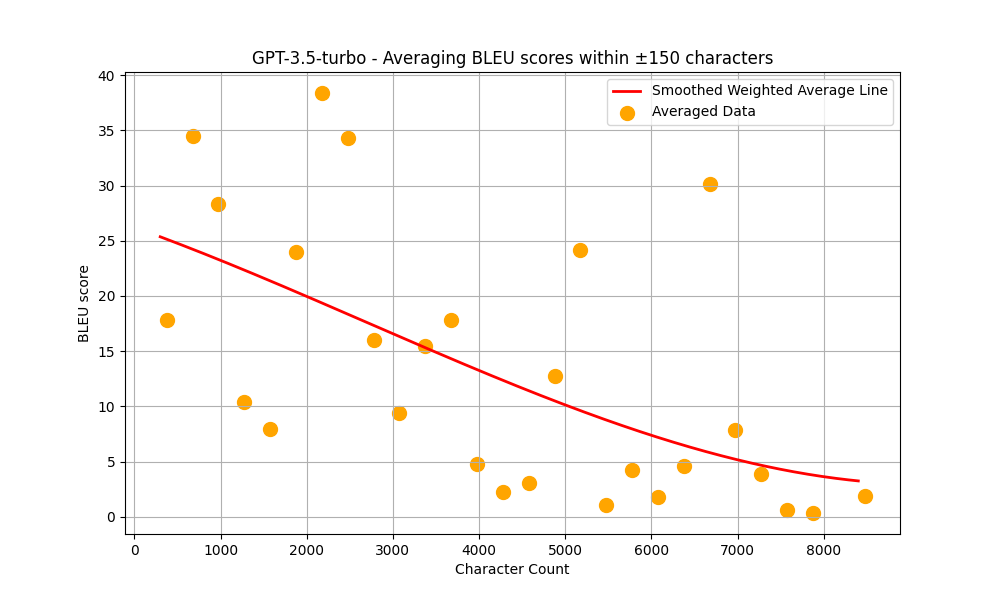
\includegraphics[width=0.95\textwidth]{obrazky-figures/docstring-gpt-bleu.png}
       \caption{\textsc{Bleu} score over character length of the input of GPT-3.5-turbo while generating docstrings.}
      \label{fig:docstring_length_gpt}
    \end{figure}

    \begin{figure}[H]
      \centering
      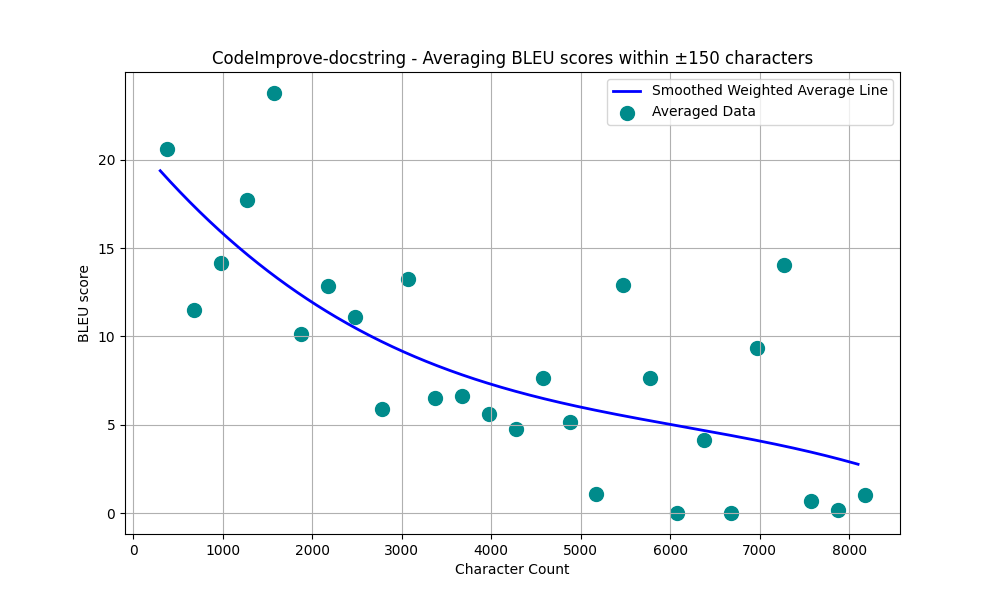
\includegraphics[width=0.95\textwidth]{obrazky-figures/Ncodeimprove-docstring.png}
       \caption{\textsc{Bleu} score over character length of the input of the CodeImprove-docstring model.}
      \label{fig:docstring_length_codeimporove}
    \end{figure}
    
    Upon human inspection, it is apparent that the quality of the docstring is much lower than the baseline. CodeImprove's docstrings are noticeably shorter than the labels.

    It is apparent that CodeImprove makes an effort to describe functions of individual parameters; however, it often fails to name them all. The model also appears to struggle with following the ordered docstring notation.

    Overall, this model does not manage to outperform the baseline either in terms of algorithmic or human evaluations.

    See examples of predictions in appendix \ref{docstr_pred}.
    
    \section{Assessment of Variable Name Generation}
    \subsection{Top3 Unigram Precision}
        Measuring the performance of variable name suggestions is somewhat nuanced. Variable names consist of several keywords, often with arbitrary word ordering.
    
        In order to take this into account when benchmarking this module, a custom variant of the traditional precision metric, dubbed \emph{Top3 Unigram precision (T3UP)}, is used. At its core, it is a ratio of the number of exact matches of unigrams $m$ between the prediction $u$ and the reference $r$ divided by either the length of the reference or the length of the prediction, whichever is greater. This way, three scores are computed from three separate predictions, and the highest one is used as the final TOP3 Unigram Precision.
        
        \begin{equation}
        \text{TOP3UP} = \max_{i=1}^{3} \left(\frac{m_i}{\max\left(\textit{length}(r), \textit{ length}(p_i)\right)}\right) \times 100
        \end{equation}
        
        The rationale for using 3 predictions to calculate the metric is that the CodeImprove extension presents the user with three choices.
        
        This approach, although simple, fits well with the nature of variable name composition, which is itself relatively primitive.

        Variable names are segmented by splitting on the boundary of a lowercase and uppercase letter to cover the camel case. A split is also performed where letters meet digits, and lastly, underscores cause a split as well to cover the snake case.

    \subsection{Performance}
        As we can see in table \ref{fig:rename_perf}, CodeImprove slightly underperformed compared to the baseline model. 
        
        \begin{table}[H]
            \centering
            \begin{tabular}{|c||c|c|}
            \hline
             & CodeImprove-rename & GPT-3.5-turbo \\
            \hline
            \hline
            TOP3UP & 35.63\,\% & \textbf{37.74\,\%} \\
            \hline
            TOP3EM & 10\,\% & \textbf{18\,\%} \\
            \hline
            \end{tabular}
            \caption{\emph{TOP3UP} is Top3 Unigram Precision, and \emph{TOP3EM} is a percentage of exact matches from 3 generated results.}
            \label{fig:rename_perf}
        \end{table}

        Results from the baseline model were extracted with a prompt specified in listing \ref{lst:rename_prompt}.
        
        \begin{lstlisting}[caption={Prompt used for sampling variable names from GPT-3.5-turbo.}, label={lst:rename_prompt}, numbers=none]
ASSISTANT:
    I am a system for generating variable names. I will accept a snippet of Python code with "<mask>" as a replacement for one of the variable names. All mask tokens hide the same variable name. I will respond with three different suggestions for what the name should be. I will consider the context of the code they are found in to generate the most accurate results. I will separate the three variable names with a comma, My output will not contain anything else but the variable names.
USER:
    < code with masked variable name >
        \end{lstlisting}

        Both models in figures \ref{fig:rename_length_gpt} and \ref{fig:rename_length_codeimporove} (note that they have different scales) show a similar curve that rises and peaks at around 2300 characters and then drops off. GPT-3.5-turbo experiences a relatively sharp drop-off, whereas CodeImprove-rename manages to retain accuracy far better and, in spite of the rising character count, only loses score linearly and quite mildly.
        
        The rise could be caused by more useful information to infer the purpose of the variable. The drop-off at higher character counts may be due to longer functions being more complex and obscure, making it more difficult to determine the purpose of individual variables.

        \begin{figure}[H]
          \centering
          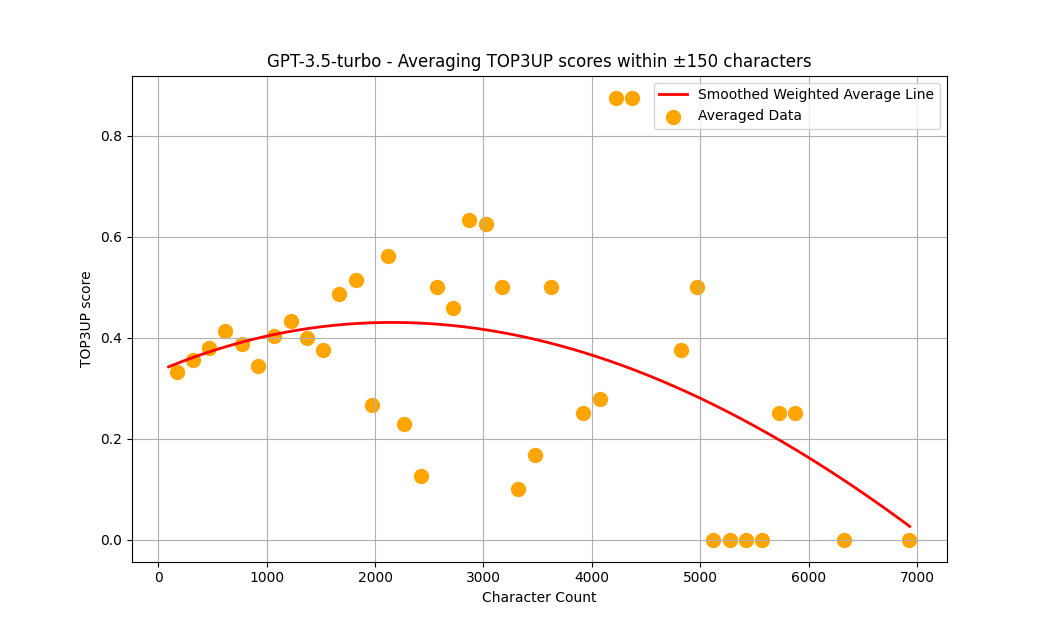
\includegraphics[width=0.85\textwidth]{obrazky-figures/gpt3turbo-rename-average.png}
           \caption{TOP3UP score over character length of the input of GPT-3.5-turbo.}
          \label{fig:rename_length_gpt}
        \end{figure}
        \begin{figure}[H]
          \centering
          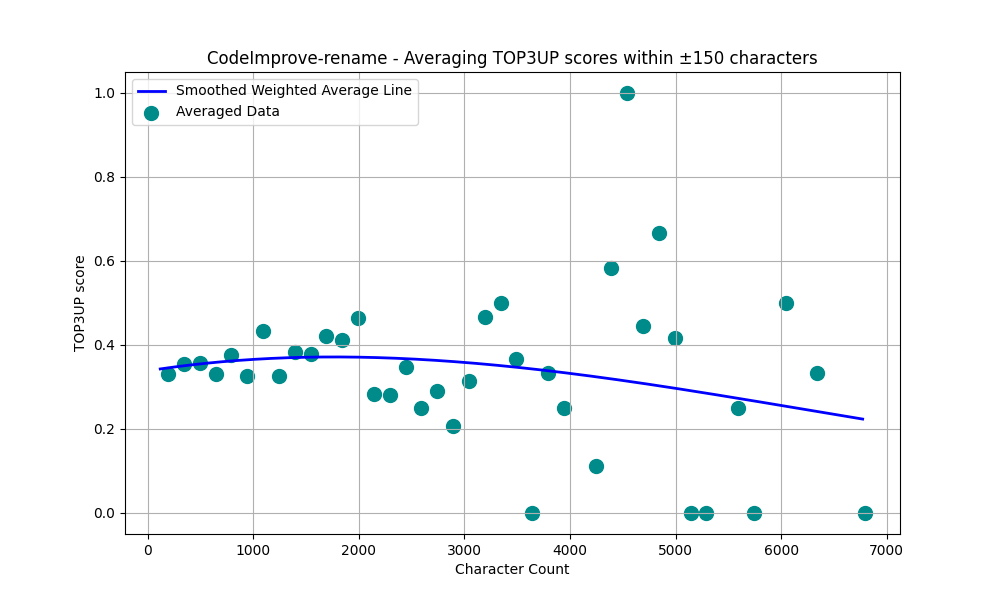
\includegraphics[width=0.85\textwidth]{obrazky-figures/codeImprove-rename-average.png}
           \caption{TOP3UP score over character length of the input of CodeImprove-rename.}
          \label{fig:rename_length_codeimporove}
        \end{figure}

        Overall, CodeImprove-rename outperforms GPT-3.5-turbo on long inputs but falls behind on shorter inputs.

        See appendix \ref{rename_pred} for examples of predictions.
        
    \section{Assessment of Error Correction}
        \subsection{LED approach}
        As mentioned in an earlier section, the LED approach to error detection proved ineffective, just from the results of the detection model; see a summary of its performance \ref{tab:error_detection}.
        \begin{table}[H]
            \centering
            \begin{tabular}{|c|c|}
            \hline
            \textbf{Error type} & \textbf{Number of samples}  \\
            \hline
            Correctly identified & 188 \\
            Incorrectly identified & 812 \\
            \hline
            \hline
            \textbf{Error lines} & \textbf{Number of samples}  \\
            \hline
            Correctly correct & 22 \\
            Partially correct & 353 \\
            All incorrect\ & 625 \\
            \hline
            \hline
            \textbf{Error presence} & \textbf{Number of samples}  \\
            \hline
            Correctly identified as \textit{no errors} & 153 \\
            Incorrectly identified as \textit{no errors} & 847 \\
            Incorrectly identified as \textit{has errors} & 863 \\
            \hline
            \end{tabular}
            \caption{Performance of the LED-based Error Detection model.}
            \label{tab:error_detection}
        \end{table}

        From closer inspection of the results, the model seems to be trying to learn the average distribution of erroneous lines, often guessing numbers in the lower ranges, which it probably learned to be a safe bet from shorter samples. However, the model does make predictions in the higher ranges as well and usually outputs numbers in the correct order. It mostly does not cross the number of the last line, though there are examples where it does.

        When it comes to detecting types of errors, the model performs similarly poorly. Most often guessing \texttt{TypeError}, though it often predicts others as well.

        In order to increase the chances of success, other approaches were modifications to the dataset explored, including variants that only included erroneous code with no false positives and only using the name of the exception class from the PyTraceBugs dataset as the error type, but the results remained similarly unsatisfactory.

        It is clear that the LED model for error detection, despite great efforts, fails to grasp the nuances of the task at hand.

        \subsection{CodeWizard approach}

        QLoRA adaptation was utilized to train the instruction-tuned CodeWizard to perform both patch-based and full code error correction. Sadly, training the LoRA layers did not yield fruits, as the model kept failing to converge even after exploring various combinations of adapter parameters. 

    
\chapter{Conclusion}
    This thesis addresses the development of a Visual Studio Code extension called CodeImprovem. The extension specifically targets the automation of comments and docstrings generation, offers suggestions for alternative variable names, and incorporates an error correction feature. It operates on function and method bodies, aiding programmers in maintaining and improving the quality and readability of their codebases.

    This work covers the basic theory and state-of-the-art practices in natural language processing. It also examines a sparse attention transformer model architecture called Longformer, which allows for the efficient processing of large sequences of code. Quantized low-rank adaptation is also explored to correct erroneous code.
    
    The extension introduced in this thesis facilitates the generation of context-specific comments and docstring, striving to help developers improve the readability of their code. It is powered by a pair of Longformer models. The suggestion of variable names is also powered by its own Longformer model. This feature aims to assist developers, particularly those who struggle creatively with naming variables. Additionally, as part of this work, a dataset containing over 16,500 samples of errors before and after patches was amassed. Despite initial attempts to implement error correction with Longformer and subsequent trials with the CodeWizard model enhanced by QLoRA, neither approach achieved the desired outcomes, producing irrelevant outputs. 
    
    The models were compared to GPT-3.5-turbo, which is a similar model used in GitHub copilot, a leading chat-based programming assistant. The docstring generator scored about 27\,\% lower \textsc{Bleu} compared to the baseline, the model for generating inline comments outperformed the baseline by about 20\,\% in \textsc{Bleu} score. The model for variable name suggestion scored about 6\,\% worse in TOP3 Unigram Precision.

    However, upon human evaluation, all three models showed results that were significantly poorer than the baseline.
    
    This work strives to create an integrated toolset that will seamlessly integrate modern advancements in machine learning into the UI and enable frictionless use of simple AI-aided tasks for operations that need to be performed most often, without the need to deal with prompts and chat windows. This goal was partially reached, leaving a lot of room for improvement. Further development should focus on including more user preference options and could use QLoRA adaptation with a larger model, which would fine-tuned multimodally and facilitate all functionality. Adding additional features would also strengthen the experience.
